% !TEX root = trkjet.tex


%%%%%%%    Centrality-RDptr distributions    %%%%%%%
The centrality dependence of \RDptr\ for two charged-particle \pt\ intervals: 1.6--2.5~\GeV\ and \mbox{6.3--10.0~\GeV}, and two different \ptjet\ ranges: 126--158~\GeV\ and 200--251~\GeV, is presented in Figure~\ref{fig:centdep}.
For both \ptjet\ selections and  1.6--2.5~\GeV\ charged particles, the magnitude of the excess increases for more central events and for \rvar\ for $\rvar < 0.3$.
The magnitude of the excess is approximately a factor of two in the most central collisions for $\rvar >$~0.3.
A continuous centrality dependent suppression of  yields of charged particles with $6.3 < \pt < 10.0$ GeV is observed.
The magnitude of the modification decreases for more peripheral collisions in both \pt\ intervals and \ptjet\ selections.

\begin{figure}[ht]
\centerline{
\begin{tabular}{cc}
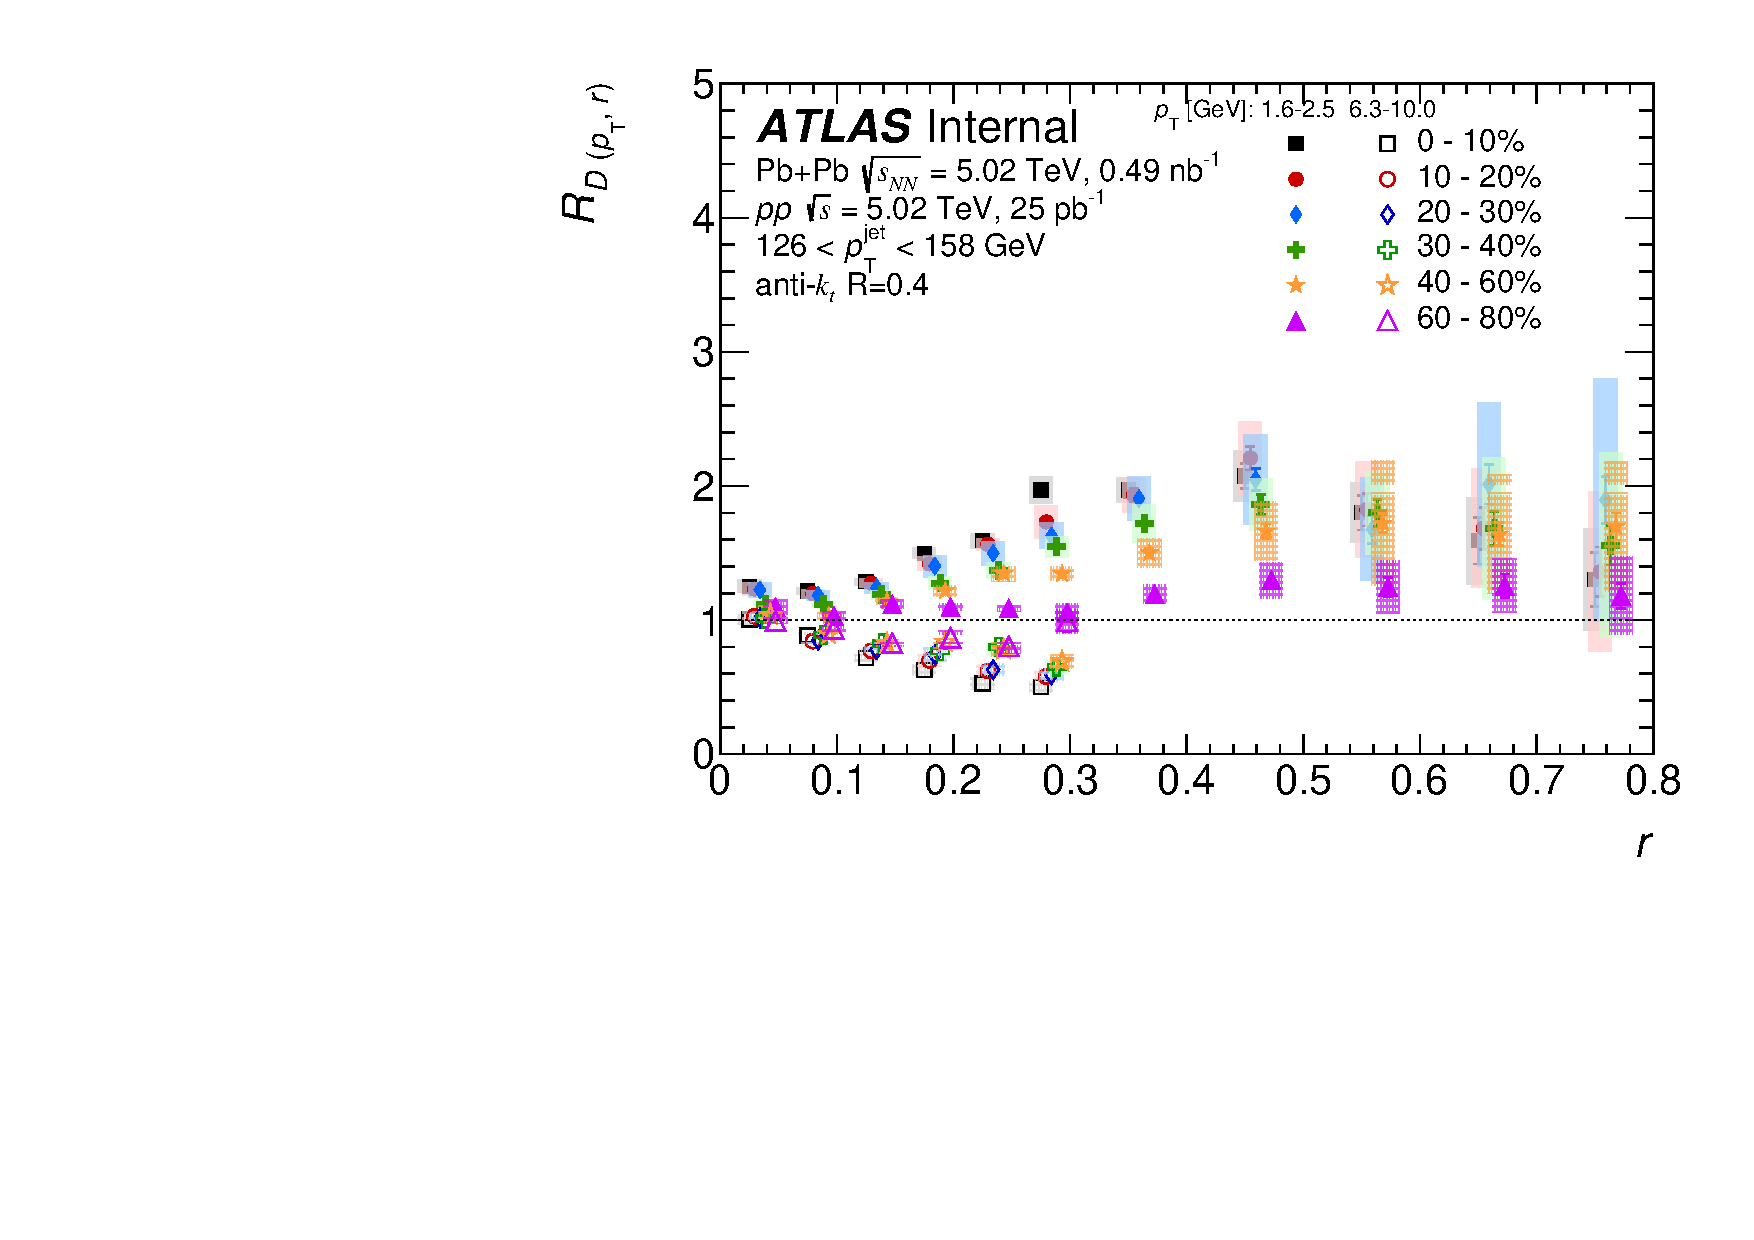
\includegraphics[width=0.36\textwidth]{figures/results/RDpT_dR_trk3_trk6_jet7} & 
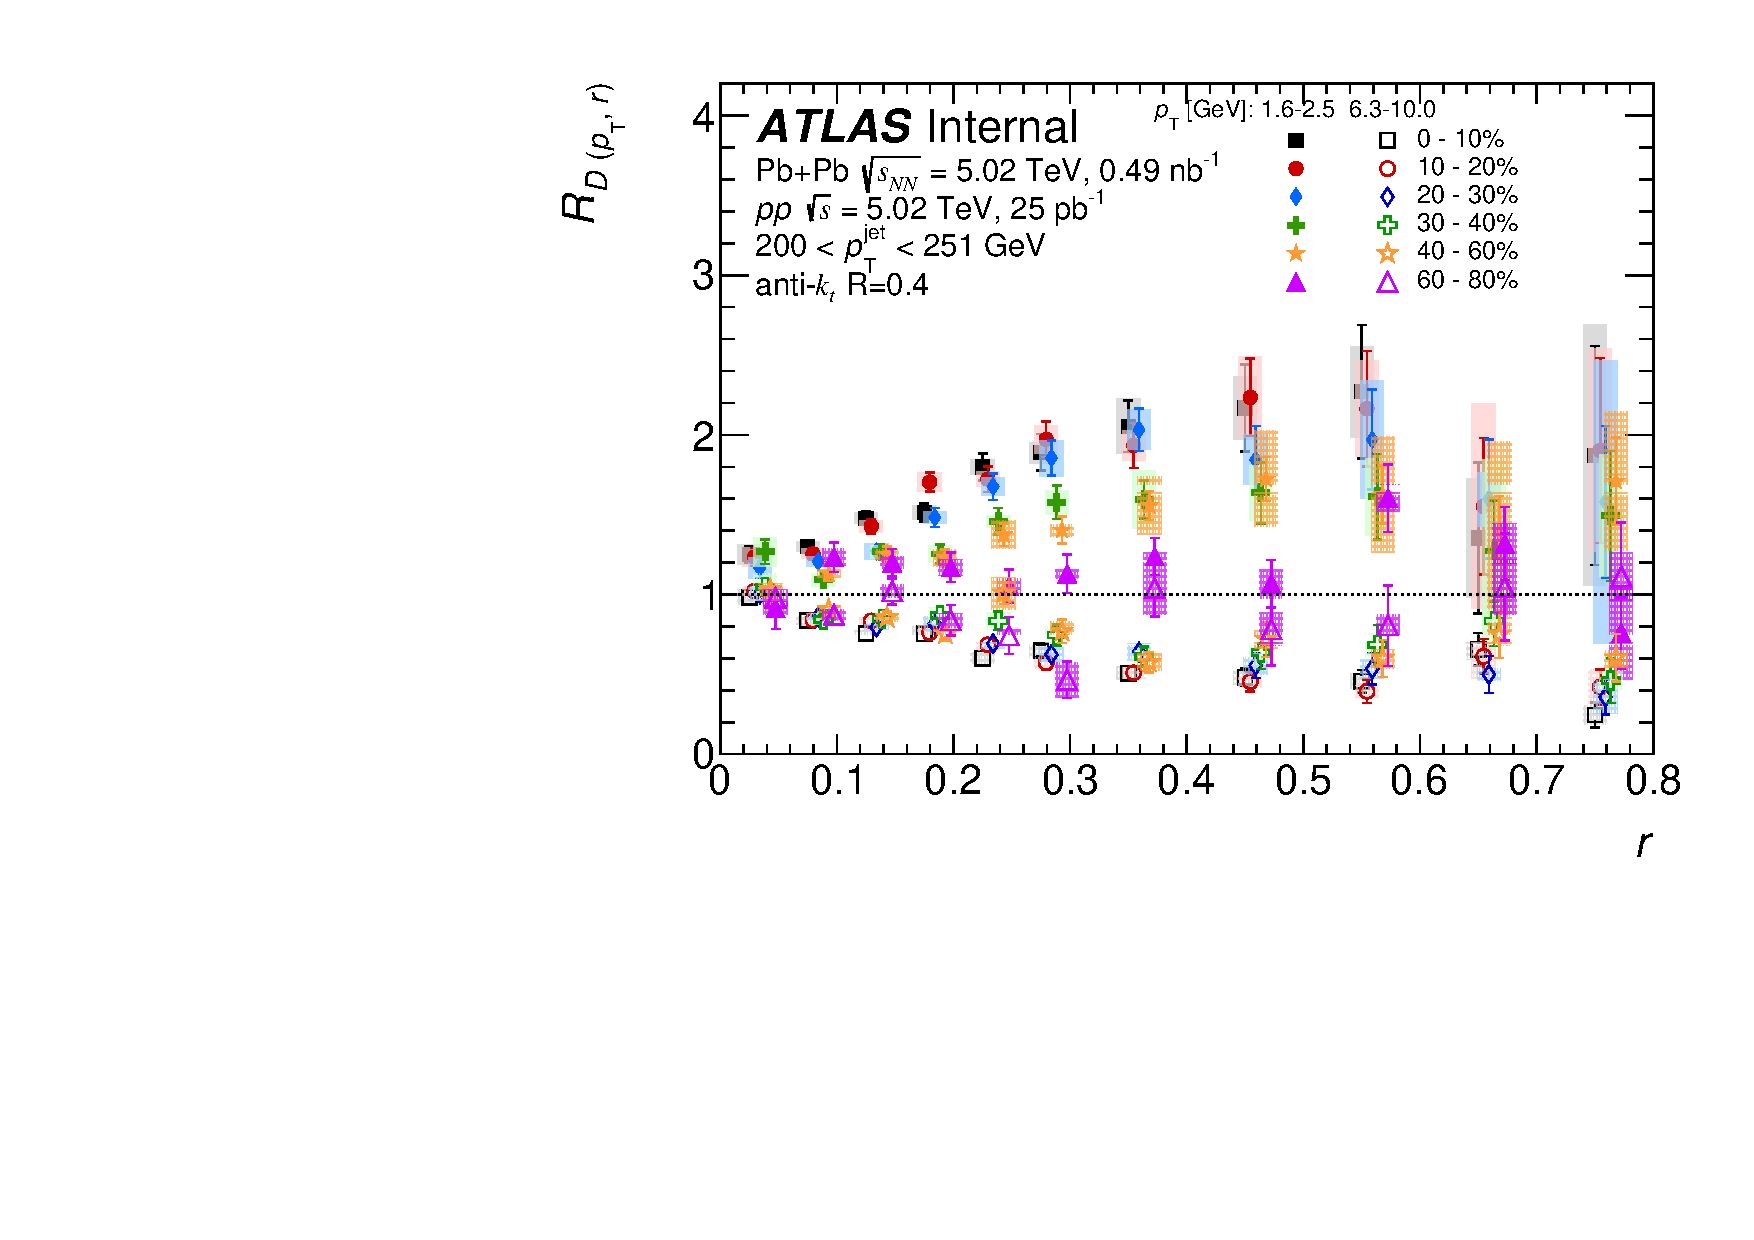
\includegraphics[width=0.36\textwidth]{figures/results/RDpT_dR_trk3_trk6_jet9} \\
\end{tabular}}
\caption{The \RDptr\ distributions for \ptjet\ of 126--158~\GeV\ (left) and 200--251~\GeV\ (right) as a function of angular distance $r$ for two \pt\ selections, 1.6--2.5~\GeV\ (closed symbols) and 6.3--10.0~\GeV\ (open symbols), and six centrality intervals.
The vertical bars on the data points indicate statistical uncertainties while the shaded boxes indicate systematic uncertainties.
The widths of the boxes are not indicative of the bin size and the points are shifted horizontally for better visibility.}
\label{fig:centdep}
\end{figure}

%%%%%%%    trkpt-RDptr distributions    %%%%%%%
%In Figure~\ref{fig:rdptr}, it was shown that for central and mid-central collisions, there is an enhancement of charged particles with $\pt <$~4.0~\GeV\ and a suppression of charged particles with $\pt >$~4.0~\GeV.
Figure~\ref{fig:pttrkdep} shows the \pt\ dependence for selections in \rvar\  for 126--158 GeV and 200--251~\GeV\ jets in the following centrality intervals: 0--10\%, 30--40\% and 60--80\%.
Interestingly, there is no significant suppression of the yields in \pbpb\ collisions for $\rvar < 0.05$ at all measured \pt.
For larger \rvar\ values the yields are enhanced for charged particles with $\pt <$~4~\GeV\ and suppressed for higher \pt\ charged particles in both the 0--10\% and 30--40\% centrality selections and both \ptjet\  ranges presented here.
The magnitude of the enhancement increases for decreasing \pt\ below 4 GeV while the suppression is enhanced with increasing \pt\ for 4--10 GeV, after which it is approximately constant.
At fixed \pt\ the magnitude of the deviation from unity is largest for $0.3< \rvar < 0.4$ and $0.5< \rvar < 0.6$.
In the 60--80\% peripheral collisions, the same trend remains true (but with smaller magnitude modifications) for \mbox{$126 < \ptjet < 158$ GeV}; for the higher \ptjet\ selection the larger uncertainties do not allow a clear conclusion to be drawn for peripheral collisions.

The enhancement of charged particles in the kinematic region of \mbox{$\pt < 4$ GeV} has two common explanations.
First, gluon radiation from the hard scattered parton as it propagates through the QGP would lead to extra soft particles \cite{Chien:2015vja, Kang:2017frl}.
Second, the interactions of a jet with the QGP and its hydrodynamic response could induce a wake that manifests itself as an enhancement of low \pt\ particles \cite{Tachibana:2017syd}.

The observed modification at \mbox{$\pt > 4$ GeV} can be explained on the basis of the larger expected energy loss of gluon-initiated jets, resulting in a relative enhancement of quark jets in \pbpb\ collisions compared to \pp\ collisions at a given \ptjet\ value~\cite{Aaboud:2018hpb, Spousta:2015fca}.
Since gluon jets have a broader distribution of particle transverse momentum with respect to the jet direction compared to quark-initiated jets \cite{OPAL:1995ab}, such an effect could describe the narrowing of the particle distribution around the jet direction for particles with $\pt >$~4.0~\GeV\ that is observed here, though no calculations of this are available.


\begin{figure}[h]
\centerline{
\begin{tabular}{ccc}
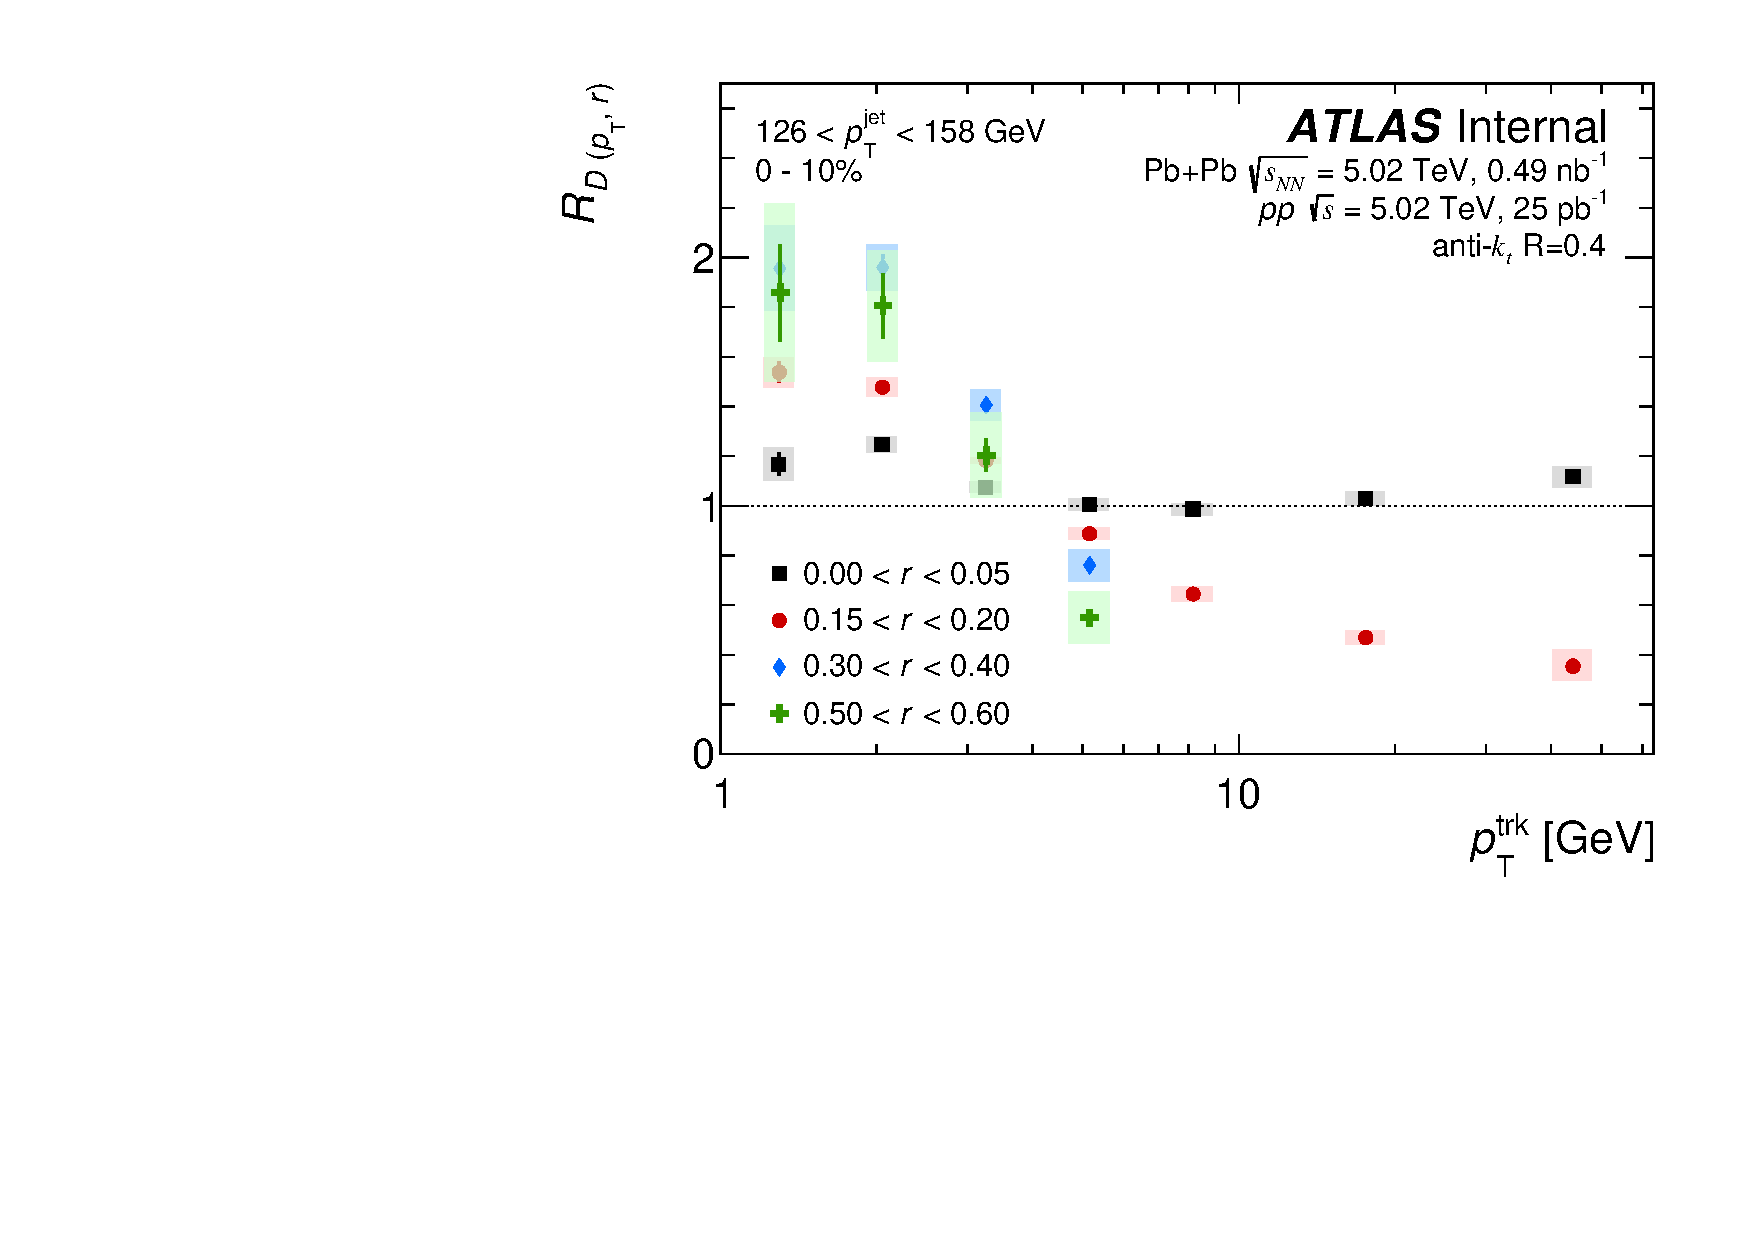
\includegraphics[width=0.36\textwidth]{figures/results/RDpT_trkpt_jet7_cent0} &
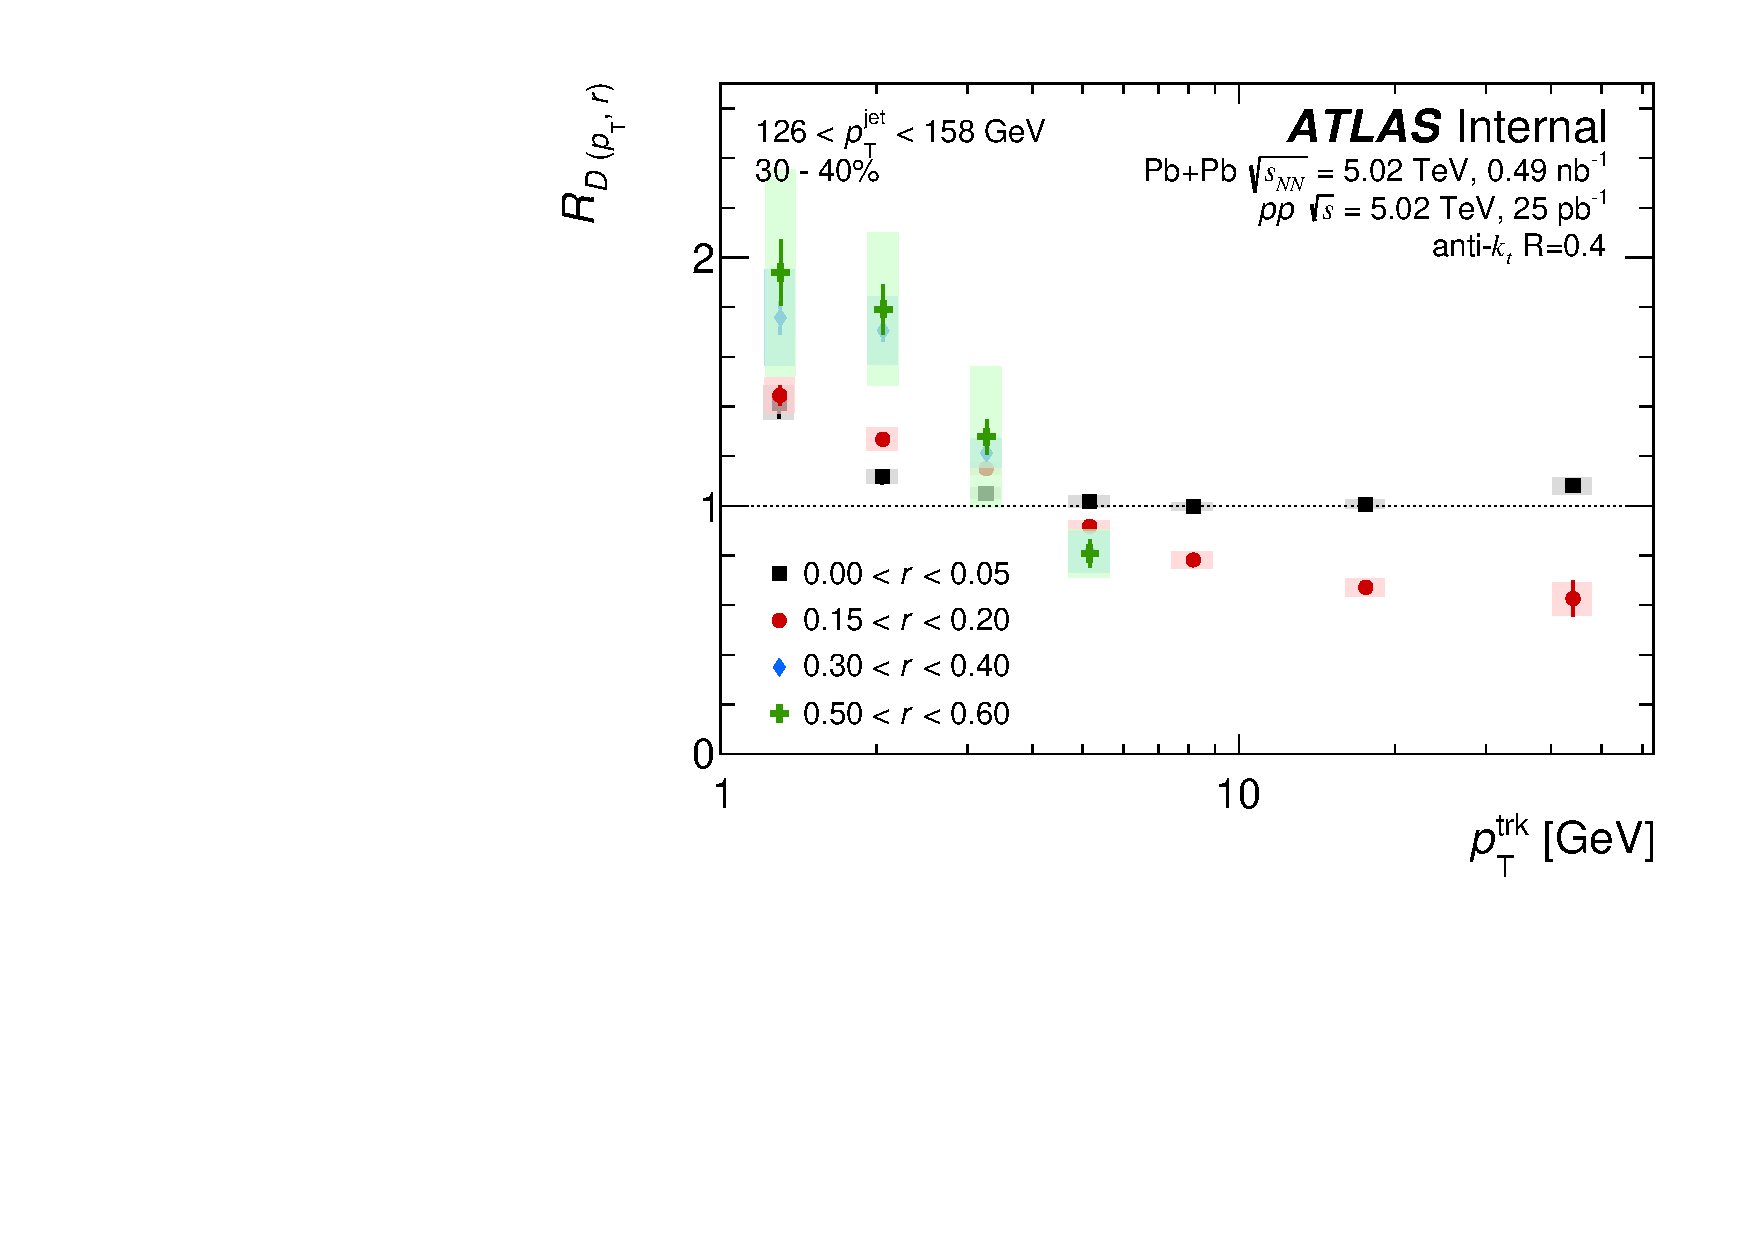
\includegraphics[width=0.36\textwidth]{figures/results/RDpT_trkpt_jet7_cent3} &
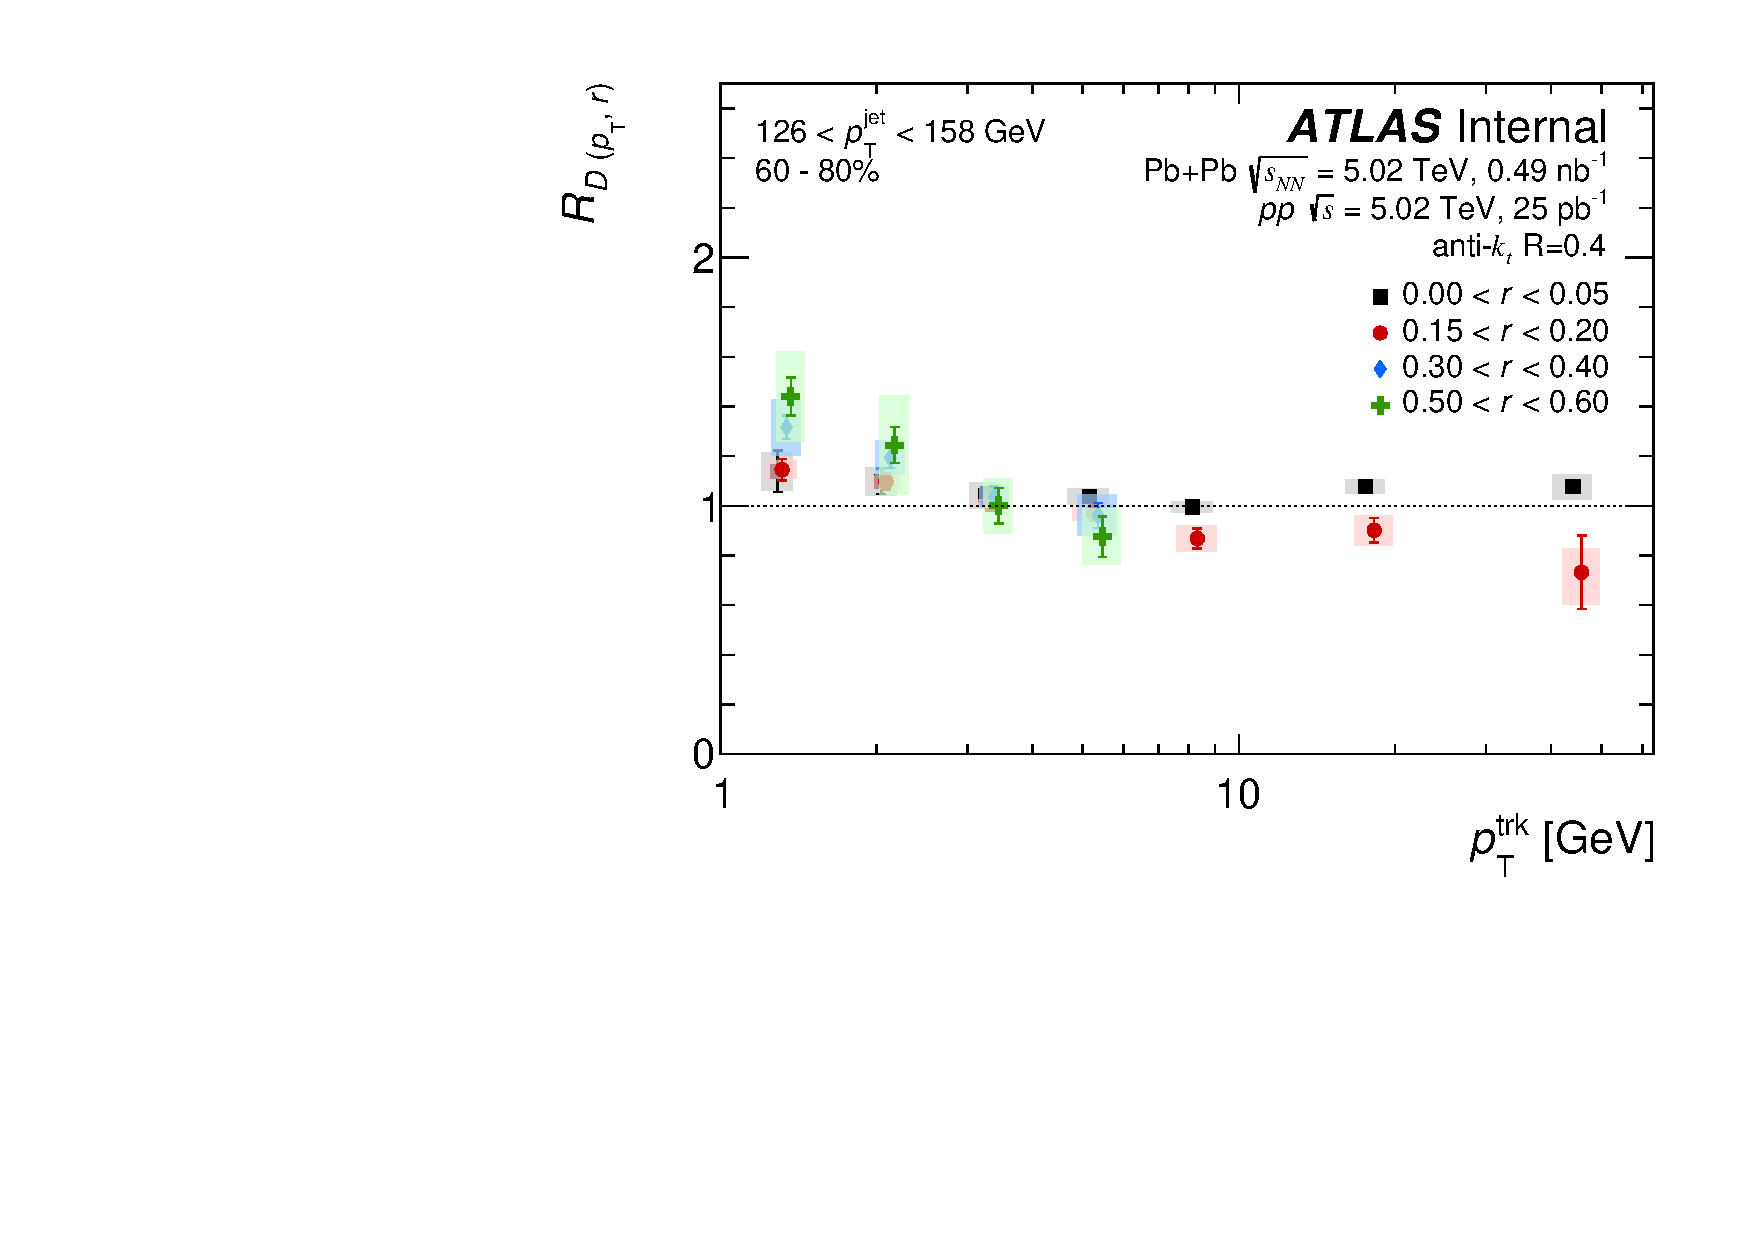
\includegraphics[width=0.36\textwidth]{figures/results/RDpT_trkpt_jet7_cent5} \\
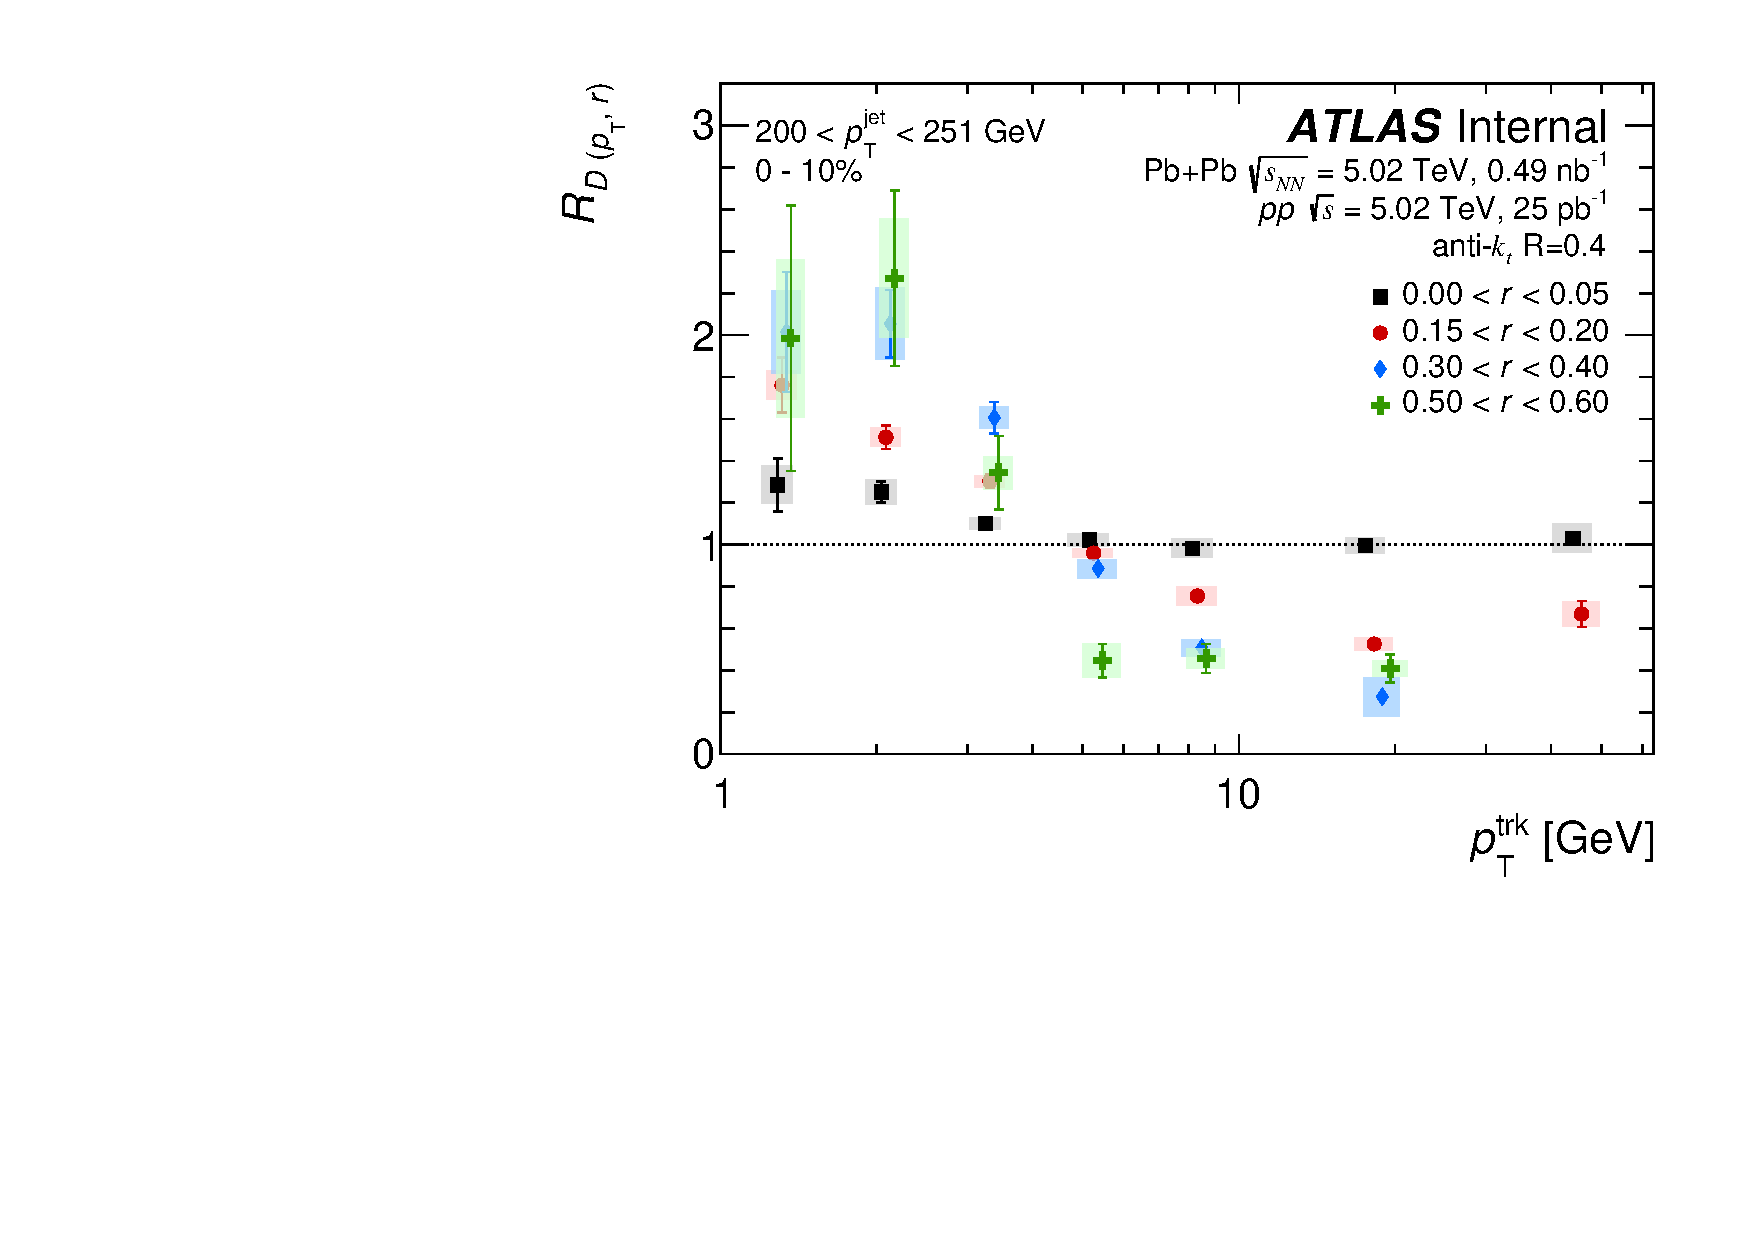
\includegraphics[width=0.36\textwidth]{figures/results/RDpT_trkpt_jet9_cent0} &
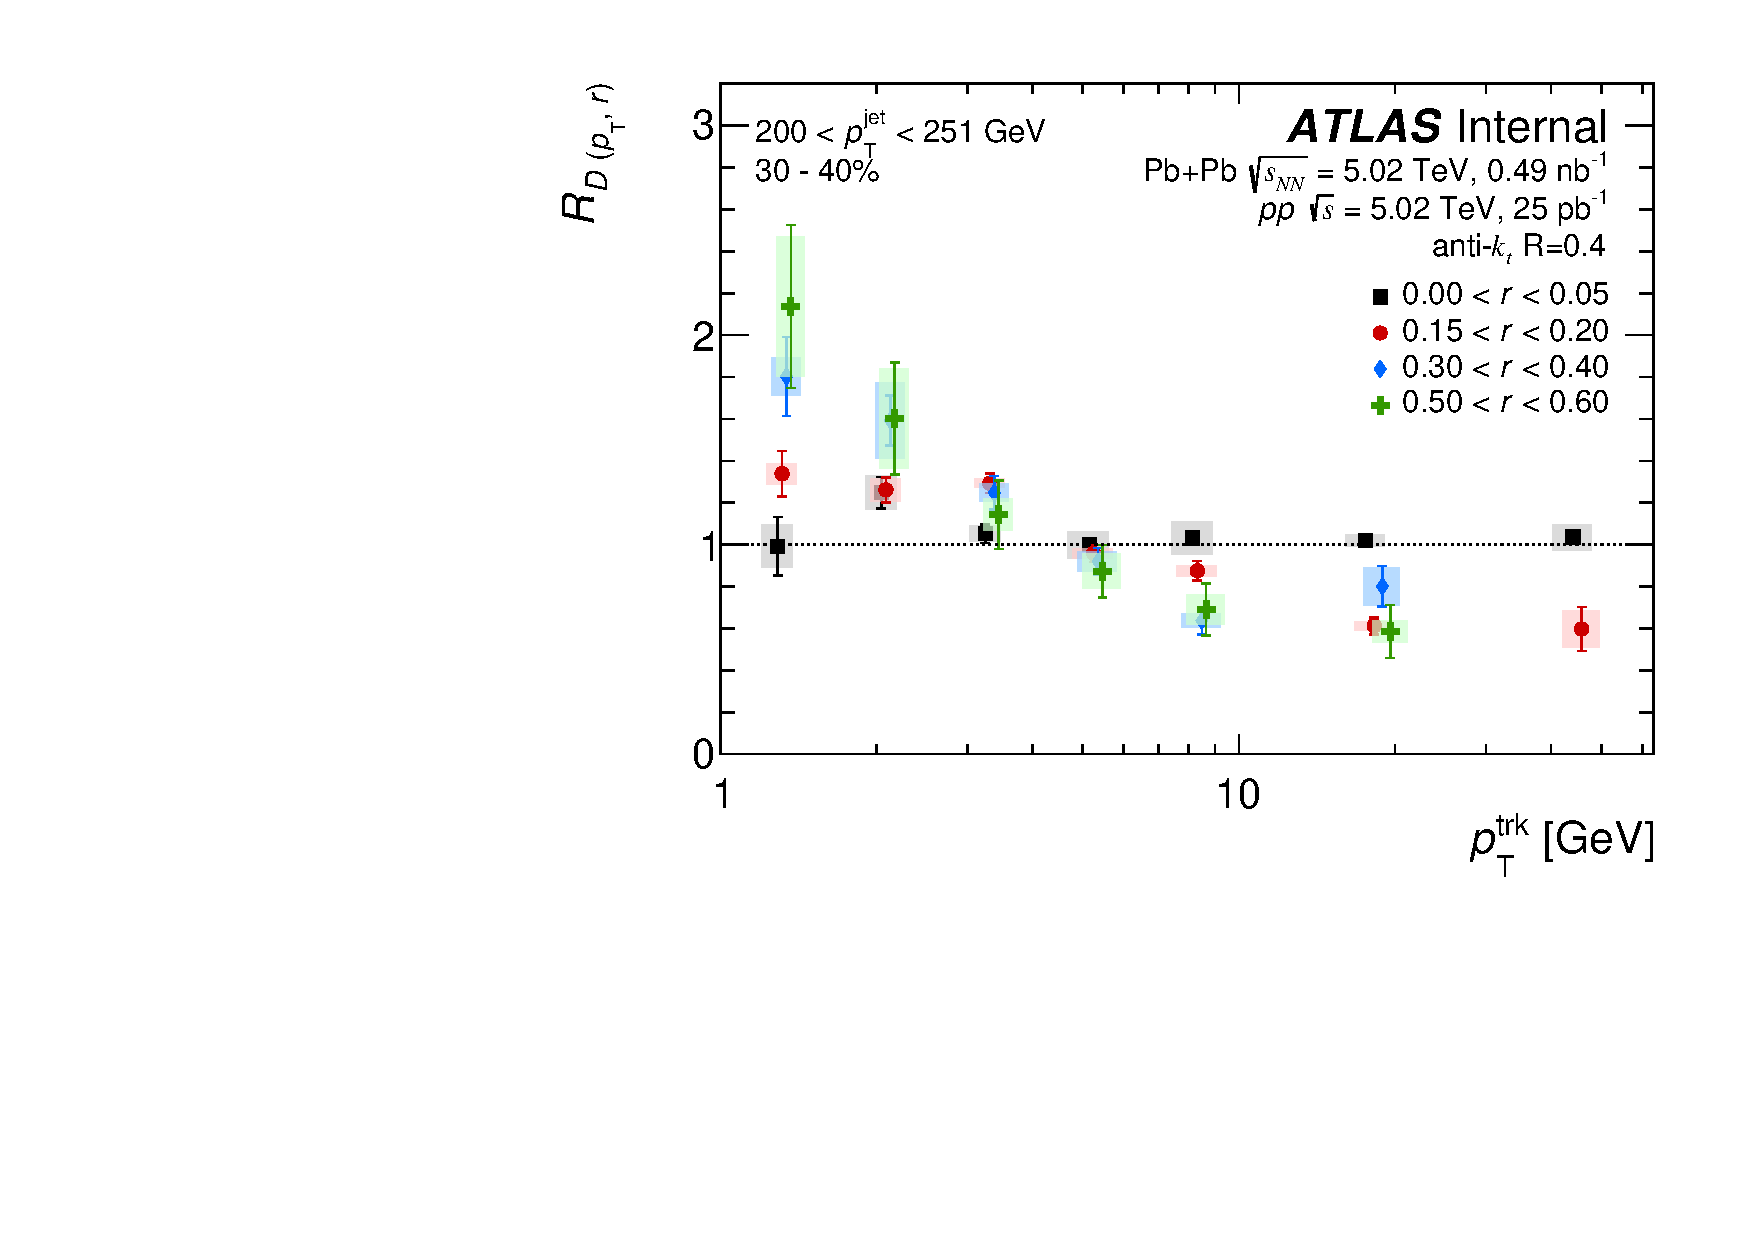
\includegraphics[width=0.36\textwidth]{figures/results/RDpT_trkpt_jet9_cent3} &
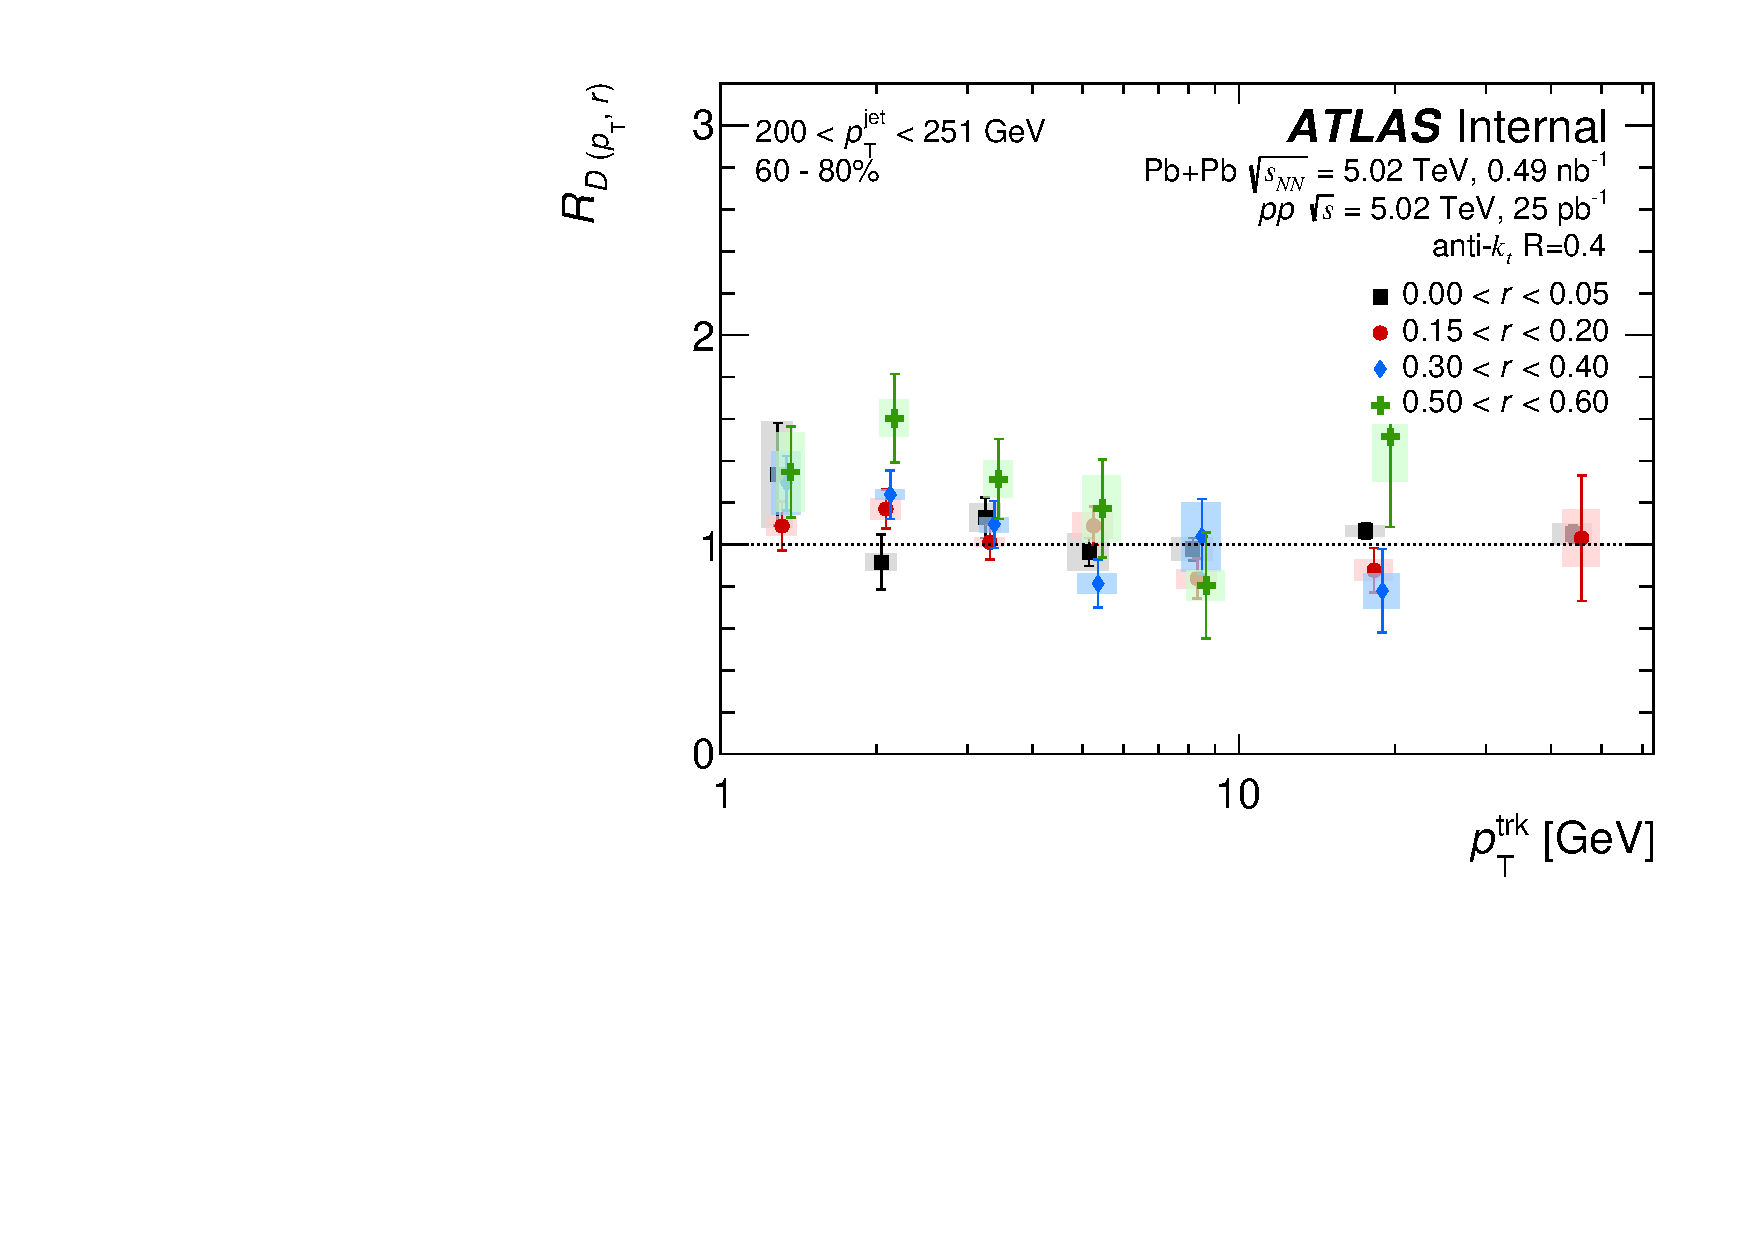
\includegraphics[width=0.36\textwidth]{figures/results/RDpT_trkpt_jet9_cent5} \\
\end{tabular}}
\caption{\RDptr\ as a function of \pt\ for  0--10\% (left), 30--40\% (middle), and 60--80\% (right) \PbPb\ collisions in two different \ptjet\ selections: 126--158~\GeV\ (top) and 200--251~\GeV\ (bottom).
The different colors indicate different angular distances from the jet axis.
The vertical bars on the data points indicate statistical uncertainties while the shaded boxes indicate systematic uncertainties.
The widths of the boxes are not indicative of the bin size and the points are shifted horizontally for better visibility.}
\label{fig:pttrkdep}
\end{figure}


%%%%%%%    Jet pT-RDptr distributions    %%%%%%%
The \RDptr\ distributions for low and high \pt\ particles in the different \ptjet\ selections are directly overlaid in Figure~\ref{fig:ptjetdep}.
These distributions are for the 0--10\% most central collisions, and show a hint of enhancement in \RDptr\ with increasing \ptjet\  for $r < 0.25$ for low  \pt\ charged particles.
No significant \ptjet\ dependence is seen at larger \rvar\ values, or for high-\pt\ charged particles at any \rvar.
This \ptjet\ dependence is further explored by defining an integral over the low \pt\ excess and is discussed in Section~\ref{sec:discussion_int}.

\begin{figure}[ht]
\centerline{
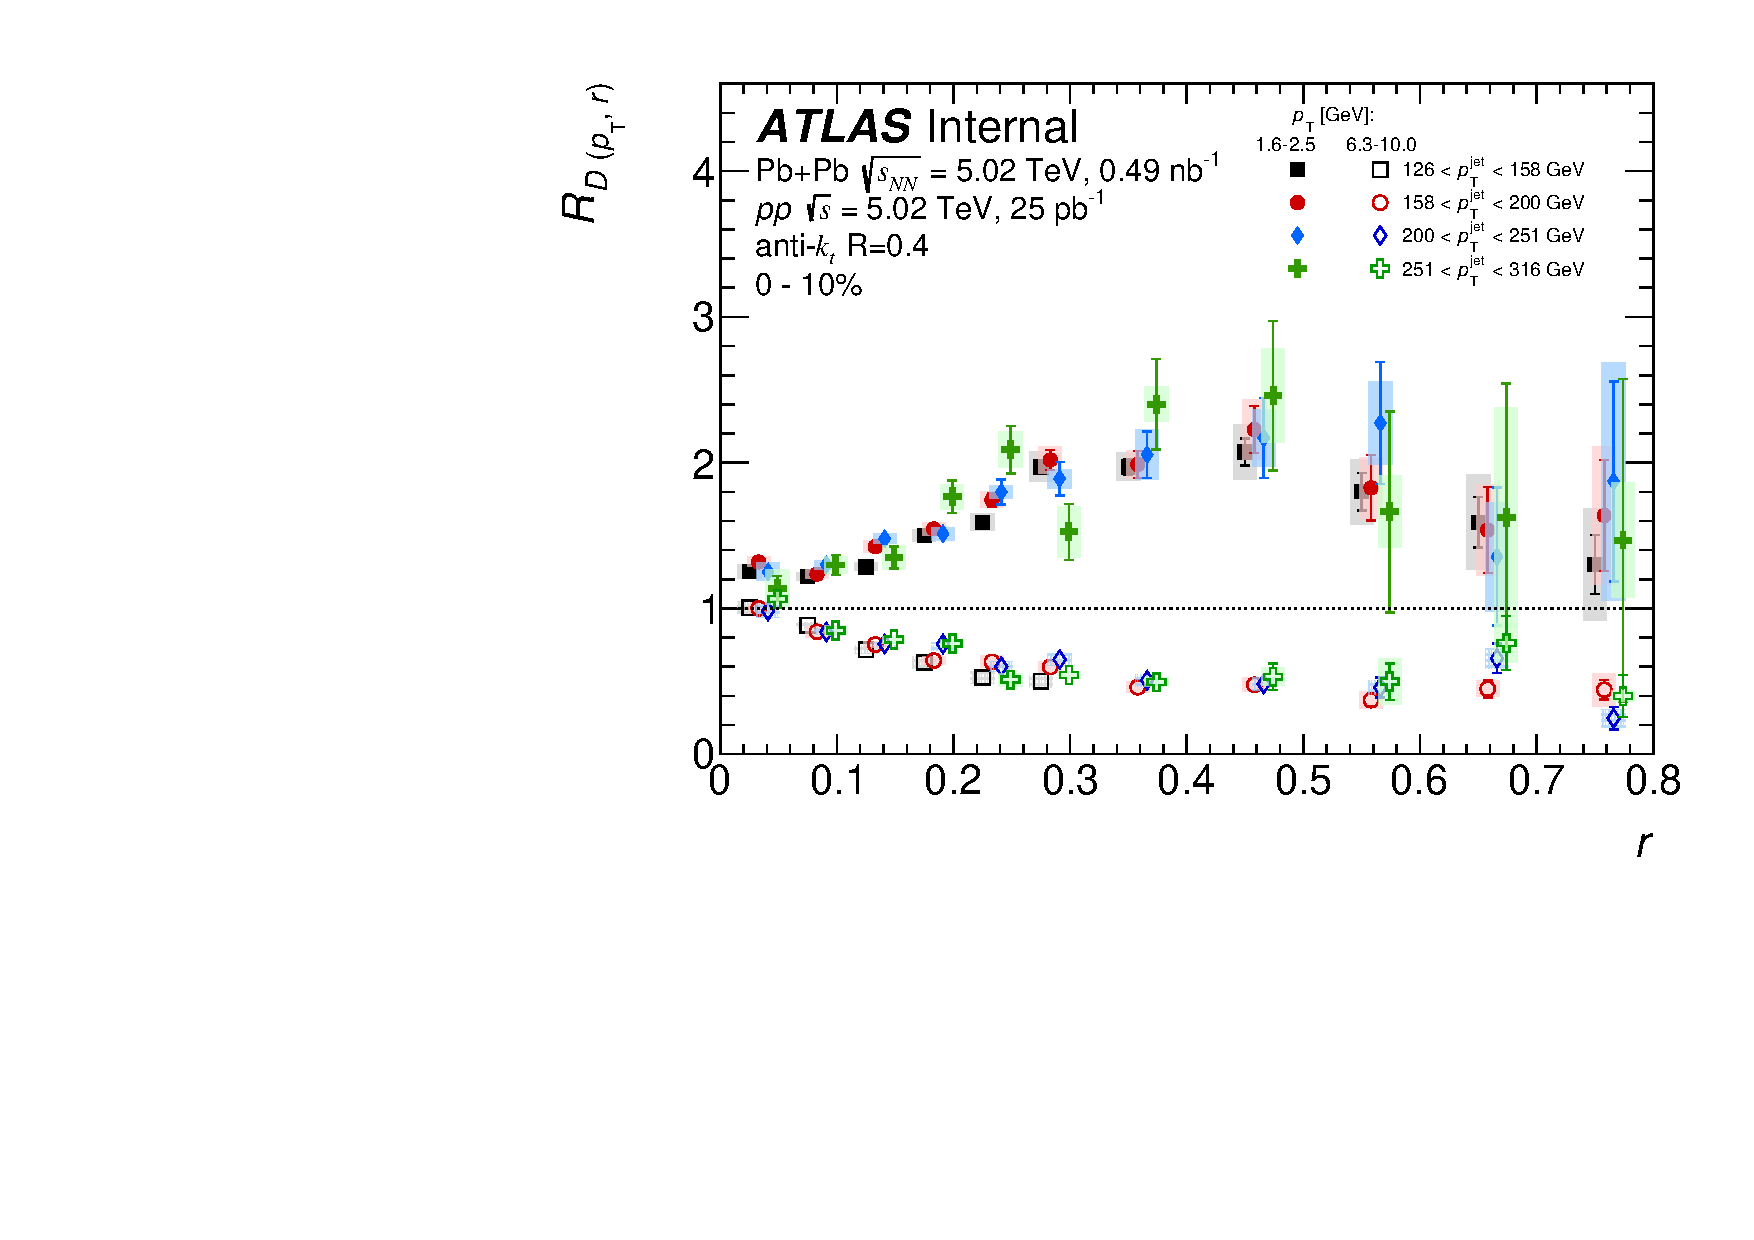
\includegraphics[width=0.36\textwidth]{figures/results/RDpT_dR_trk3_trk6_cent0}}
\caption{\RDptr\ as a function of \rvar\ for 0--10\% collisions for charged particles with 1.6~$< \pt <$~2.5~\GeV\ (closed symbols) and 6.3~$< \pt <$10.0~\GeV\ (open symbols) for different \ptjet\ selections.
The vertical bars on the data points indicate statistical uncertainties while the shaded boxes indicate systematic uncertainties.
The widths of the boxes are not indicative of the bin size and the points are shifted horizontally for better visibility.}
\label{fig:ptjetdep}
\end{figure}



%%%%%%%    Delta DPtr distributions    %%%%%%%
\subsection{\DeltaDptr\ distributions}
\label{sec:delta_dptr}
In addition to the ratios of the \Dptr\ distributions, differences between the unfolded charged-particle yields are also evaluated as \DeltaDptr\ to quantify the modification in terms of the particle density.

These differences are presented as a function of $r$ for different \pt\ selections in 0--10\% central collisions in Figure~\ref{fig:deltadptr}.
These distributions show an excess in the charged-particle yield density for \pbpb\ collisions compared to \pp\ collisions for charged particles with $\pt <4.0$ GeV.
This ranges from 0.5 to 4 particles per unit area per GeV for 1 \GeV\ charged particles in 126--158~\GeV\ jets for 0--10\% central \pbpb\ collisions and increases with increasing \ptjet.
The largest excess for charged particles with $\pt <$~4.0~\GeV\ is within the jet cone.
For large \rvar\ values, the difference decreases, but remains positive.
A depletion for higher \pt\ particles of approximately 0.5 particles per unit area per GeV is seen for 126--158~\GeV\ jets in 0--10\% central \pbpb\ collisions.
The magnitude of this depletion increases for higher \ptjet.
There is a minimum in the \DeltaDptr\ distributions of charged particles with \mbox{$ 4.0 < \pt <  25.1$}~\GeV\ at $0.05 < \rvar < 0.10$ that is seen at many \ptjet\ ranges under investigation.
The magnitudes of the excesses and deficits discussed here are dependent on the selected charged-particle \pt.

\begin{figure}
\centerline{
\begin{tabular}{cc}
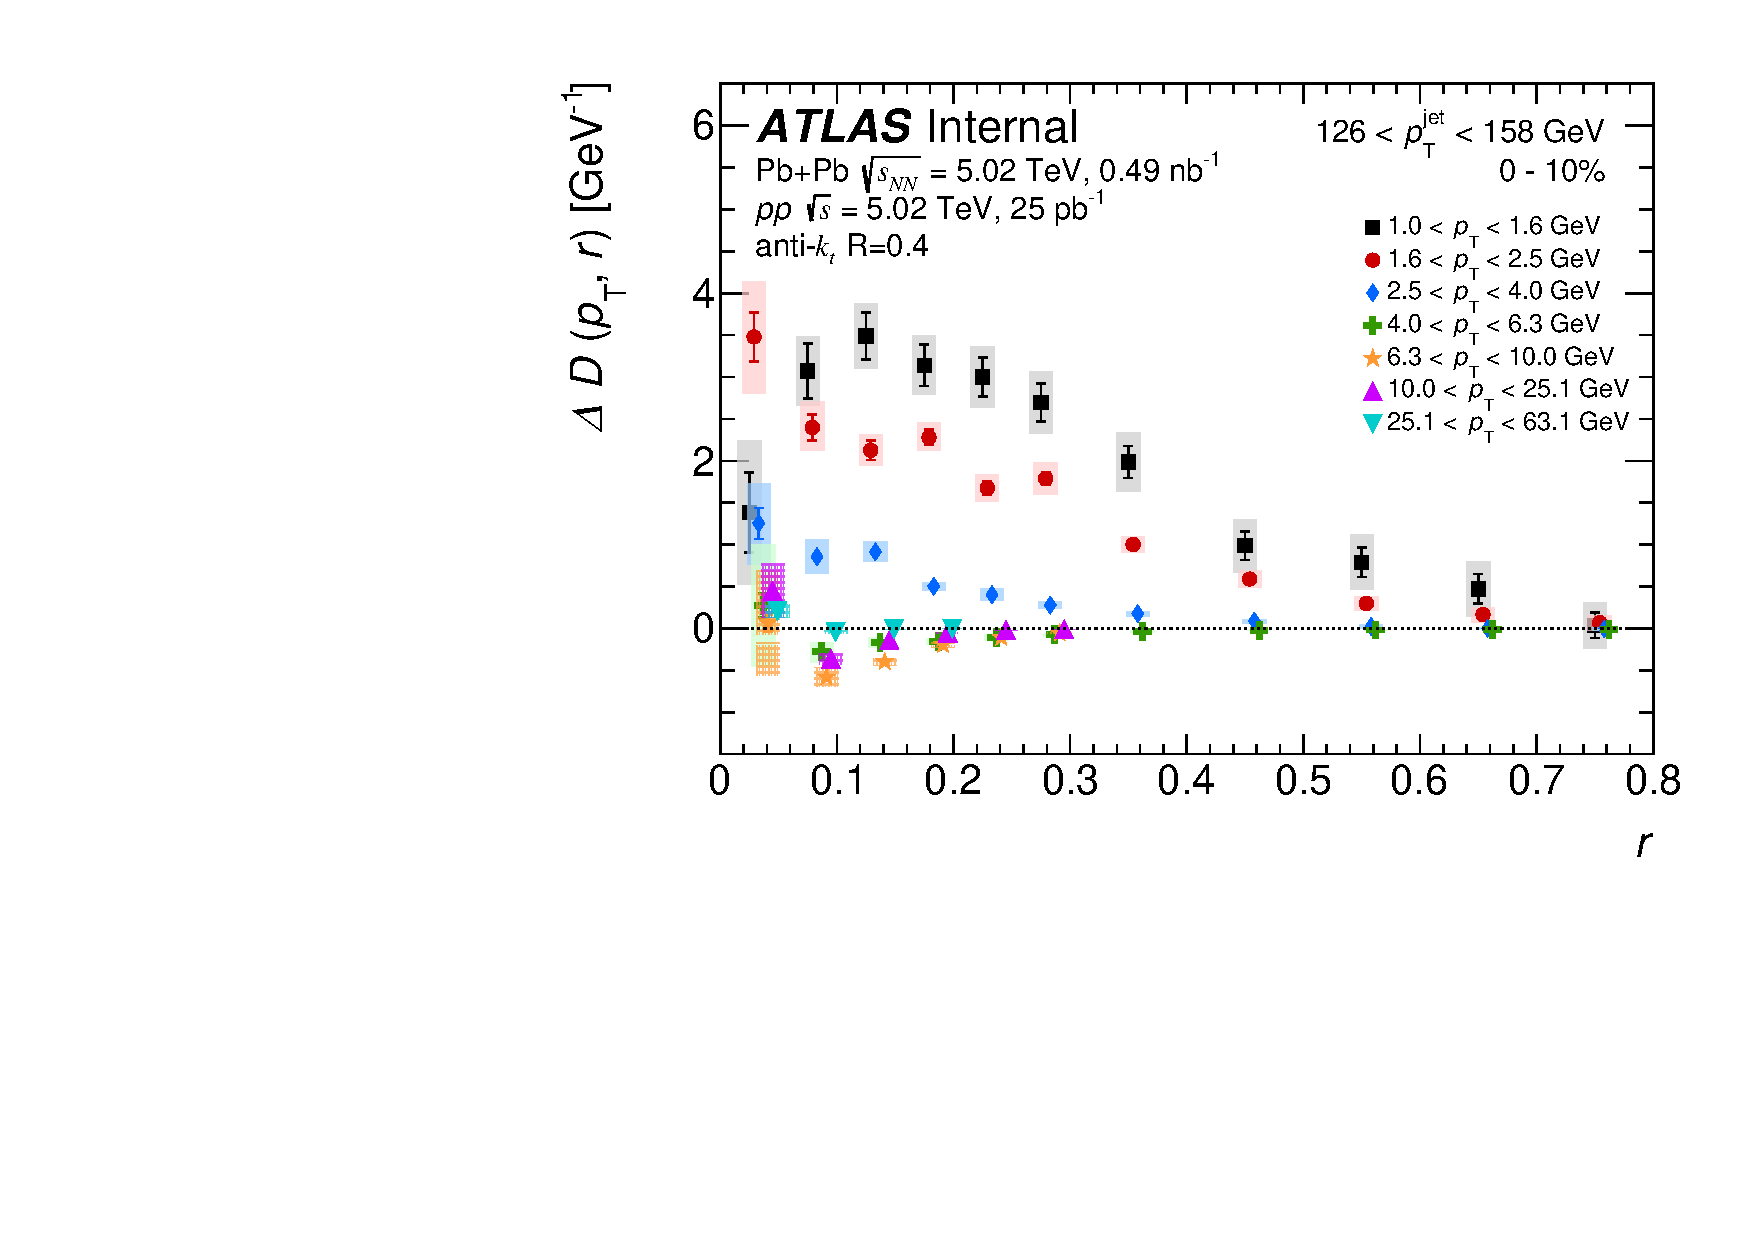
\includegraphics[width=0.36\textwidth]{results/DeltaDpT_dR_jet7_cent0} &
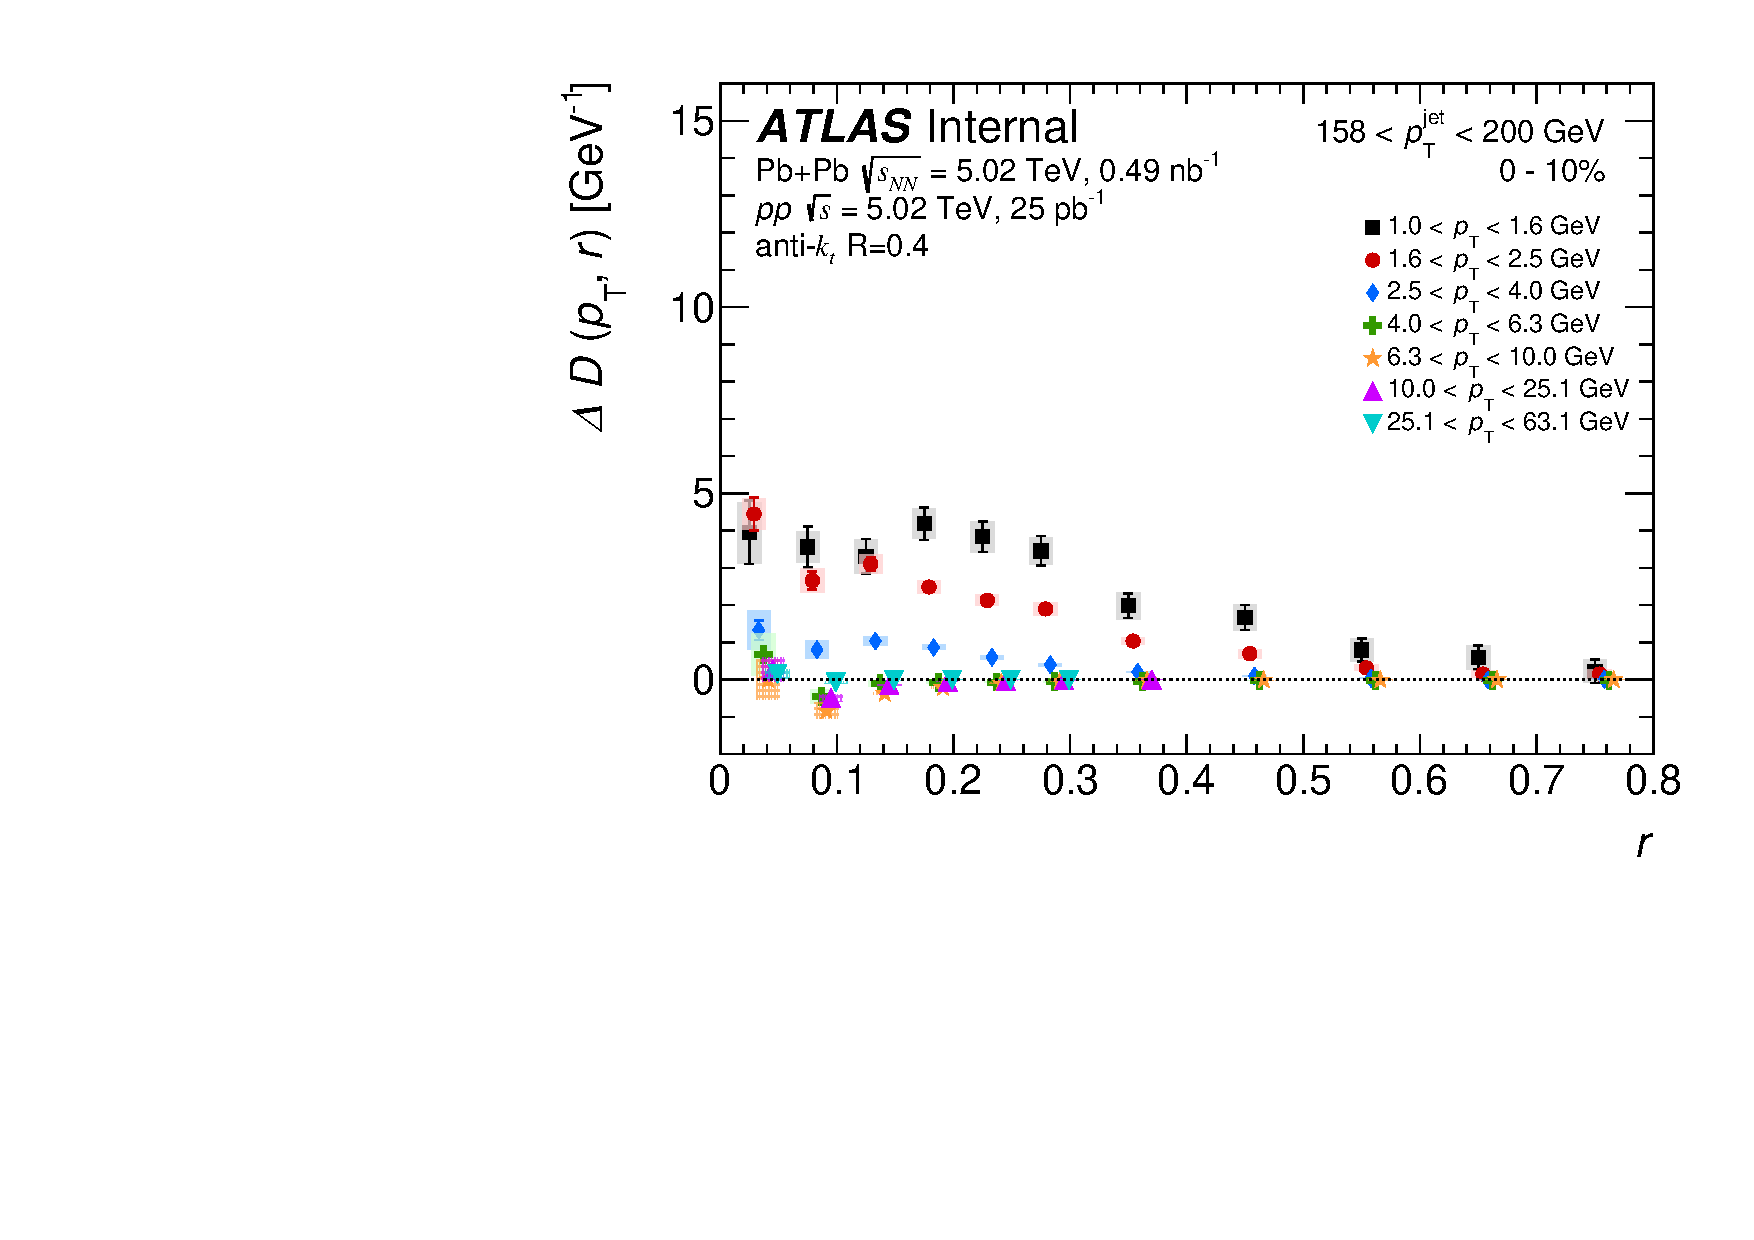
\includegraphics[width=0.36\textwidth]{results/DeltaDpT_dR_jet8_cent0} \\
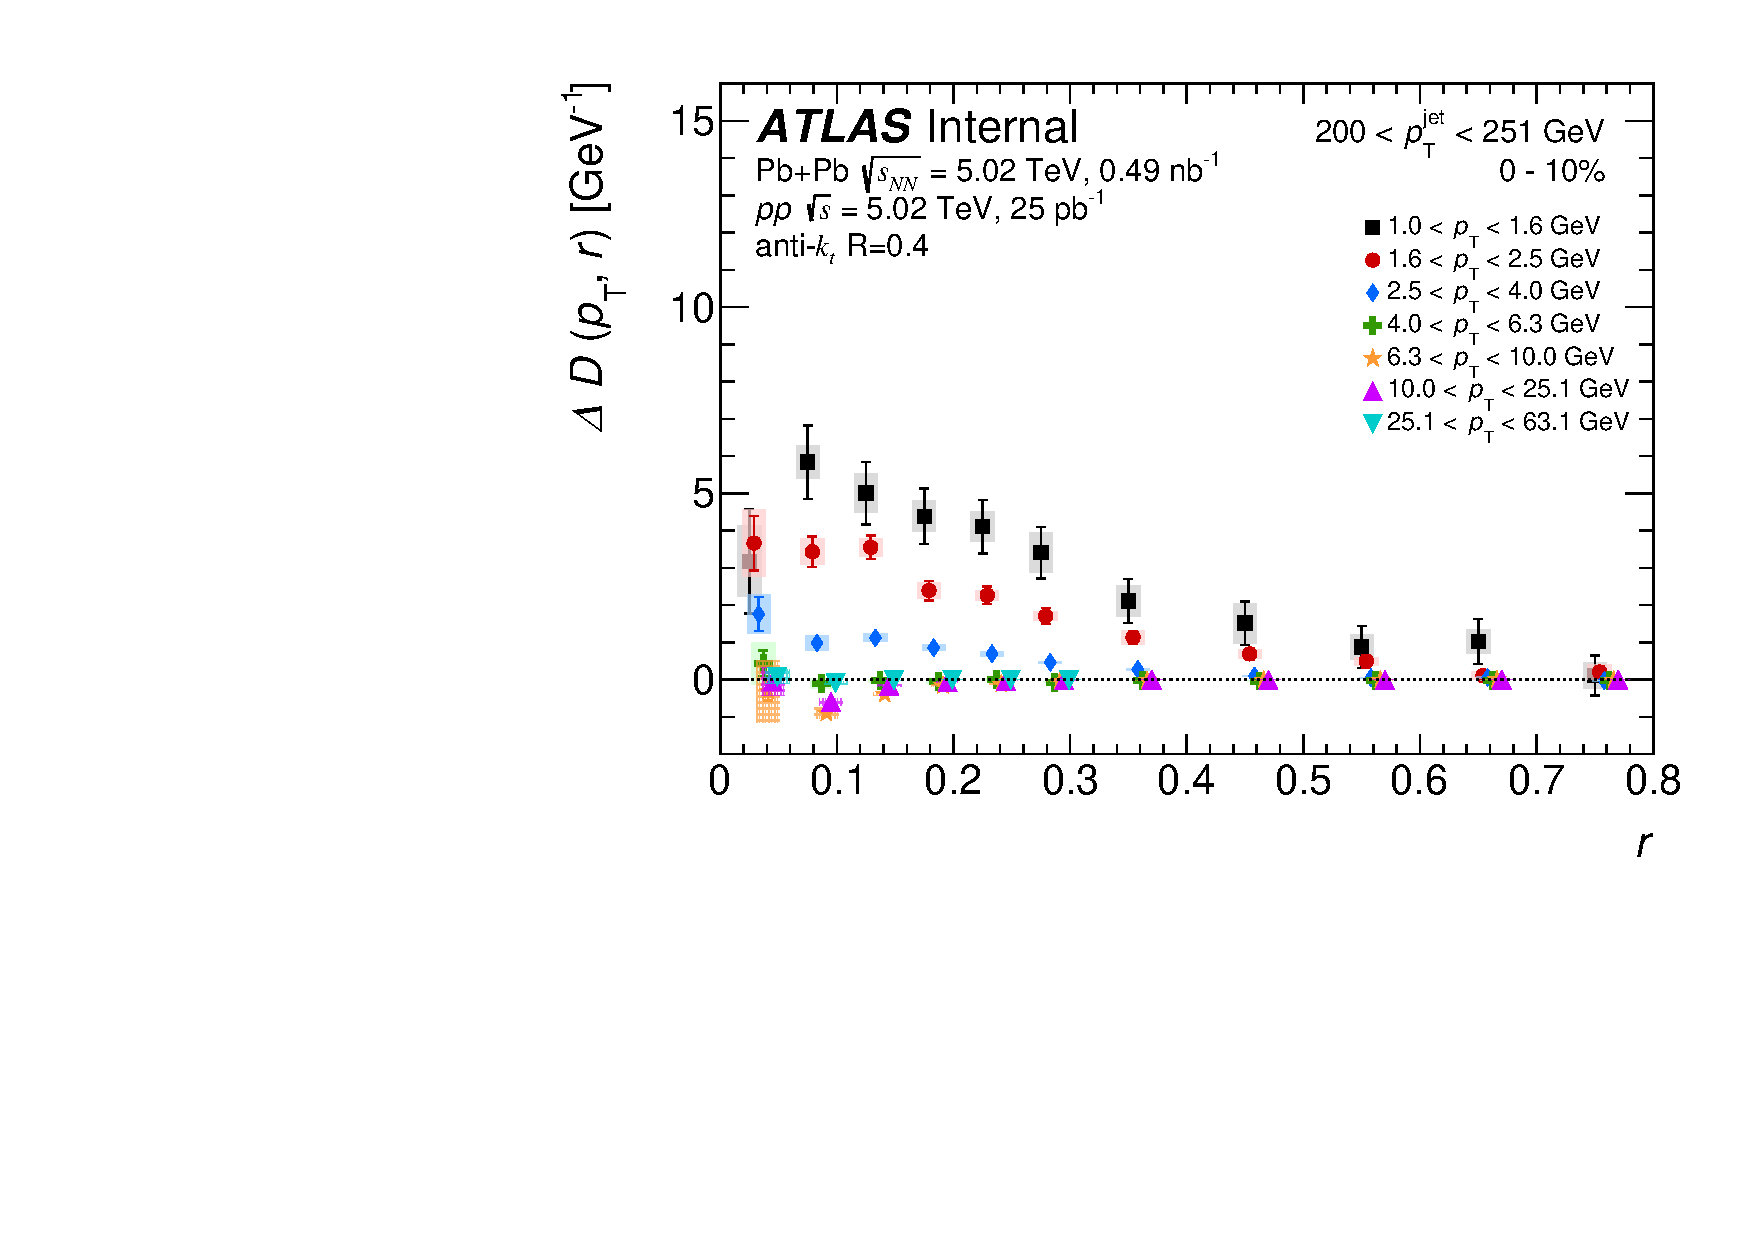
\includegraphics[width=0.36\textwidth]{results/DeltaDpT_dR_jet9_cent0} &
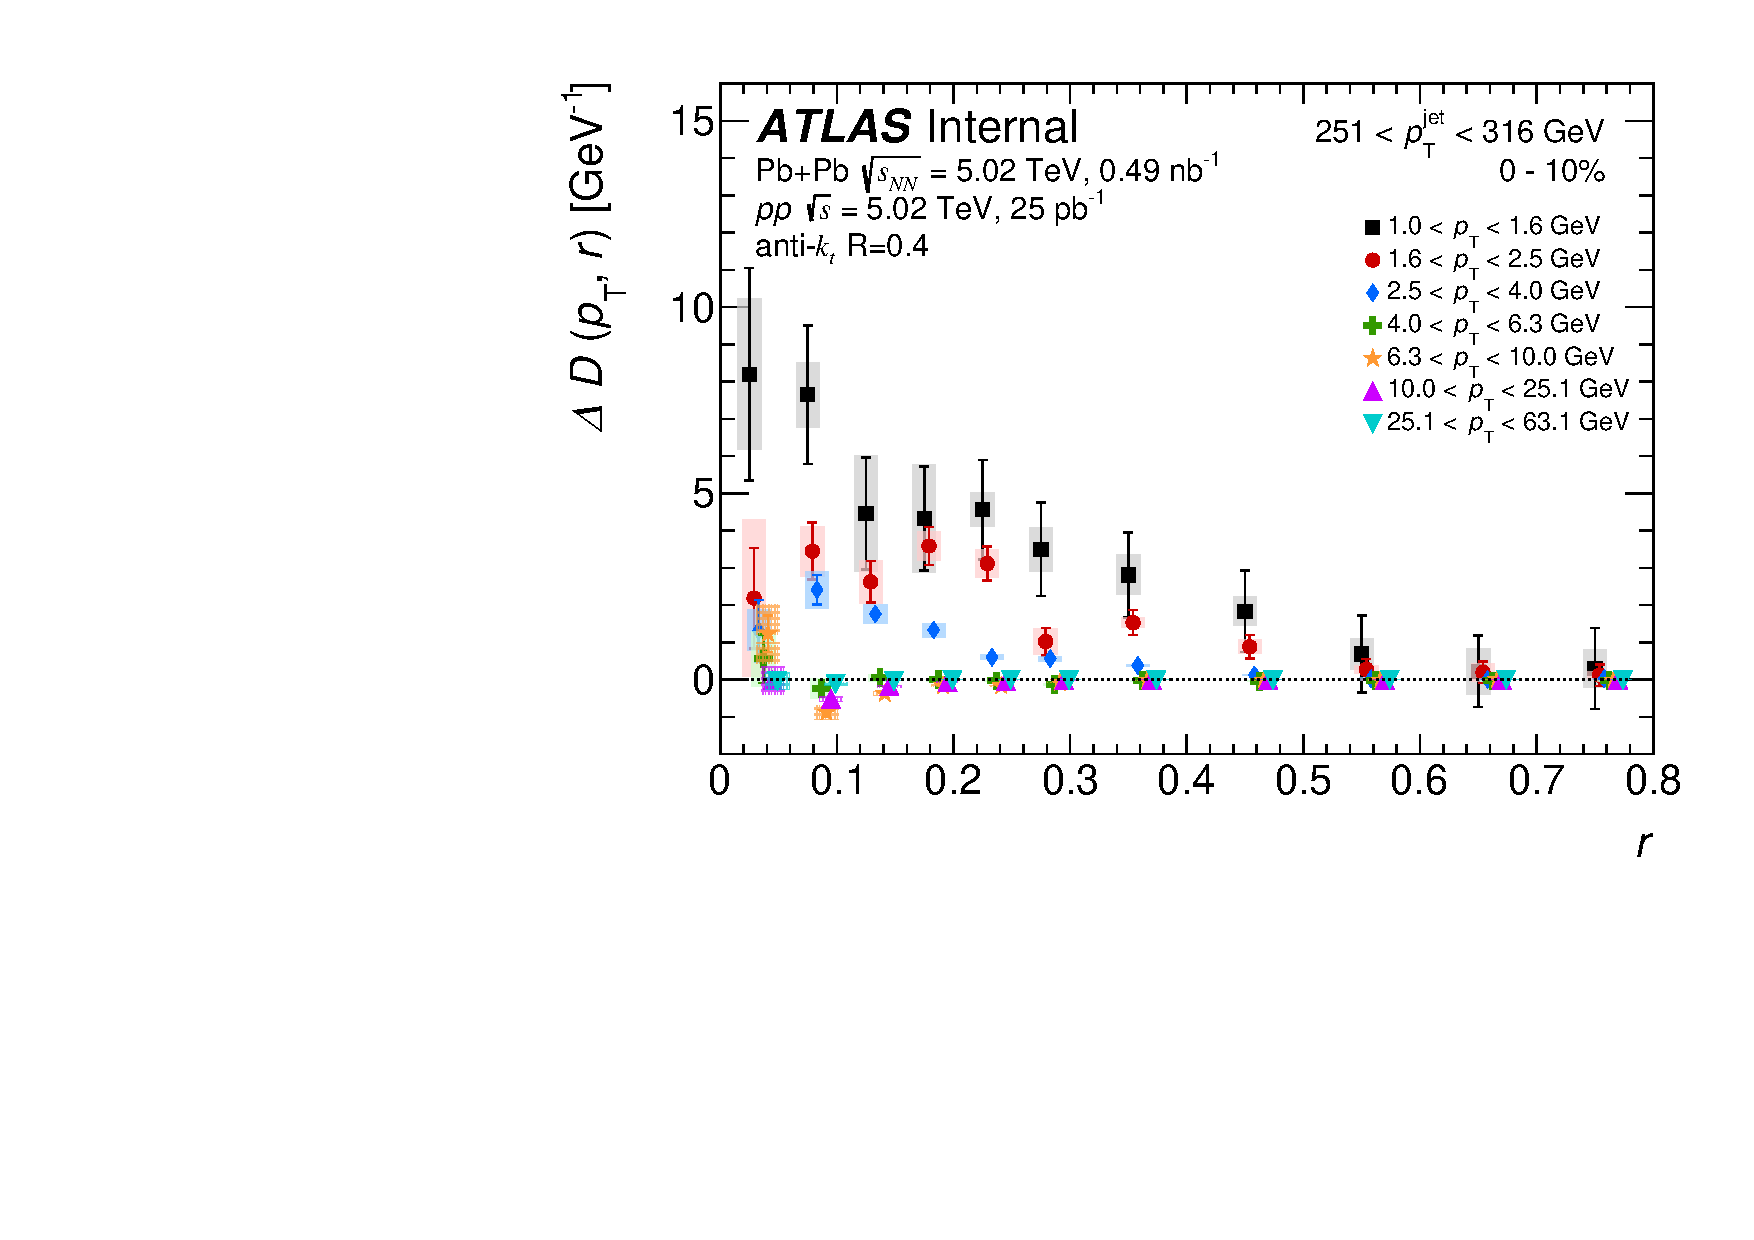
\includegraphics[width=0.36\textwidth]{results/DeltaDpT_dR_jet10_cent0} \\
\end{tabular} }
\caption{\DeltaDptr\ as a function of \rvar\ in central collisions for all \pt\ ranges in four \ptjet\ selections: 126--158~\GeV, 158--200~\GeV, 200--251~\GeV, and 251--316~\GeV.
The vertical bars on the data points indicate statistical uncertainties while the shaded boxes indicate systematic uncertainties.
The widths of the boxes are not indicative of the bin size and the points are shifted horizontally for better visibility.}
\label{fig:deltadptr}
\end{figure}





%%%%%%%%%%%%%
\subsection{\pt\ integrated distributions}
\label{sec:discussion_int}
Motivated by similar studies of the enhancement of soft fragments in jet fragmentation functions in \pbpb\ compared to \pp\ collisions from Ref.~\cite{Aaboud:2018hpb}, the unfolded \Dptr\ distributions are integrated for charged particles with \pt\ < 4 GeV to construct the quantities $\Theta(\rvar)$ and $P(\rvar)$ defined as:

\begin{align*}
\Theta(\rvar) &= \int_{1 \text{ GeV}}^{4 \text{ GeV}} \Dptr  \fd \pt \\
P(\rvar) &= \int_0^r \int_{1 \text{ GeV}}^{4 \text{ GeV}} D(\pt, r') \fd \pt \fd r'
\end{align*}
The $\Theta(\rvar)$ values are integrated over the charged-particle \pt\ interval of 1--4~\GeV\ to provide a summary look at the \pt\ region of enhancement discussed above.
The $P(\rvar)$ values further add a running integral over \rvar\ and provide information about the jet shape.
Both of these quantities are compared between the \pp\ and \pbpb\ systems to give the following distributions:

\begin{align*}
\Delta_{\Theta(\rvar)} &= \Theta(\rvar)_{\mathrm{Pb+Pb}} - \Theta(\rvar)_{pp} \\
R_{\Theta(\rvar)} &= \frac{\Theta(\rvar)_{\mathrm{Pb+Pb}}}{\Theta(\rvar)_{\mathrm{pp}}} \\
R_{P(\rvar)} &= \frac{P(\rvar)_{\mathrm{Pb+Pb}}}{P(\rvar)_{pp}}
\end{align*}
These integrated quantities are intended to provide some summary information about the location with respect to the jet axis, magnitude, and \ptjet\ dependence of the low-\pt\ charged-particle excess discussed above.
The ratio quantities are useful for comparisons to other \pbpb\ measurements; $\Delta_{\Theta(\rvar)}$ is very similar to $\DeltaDptr$, however it is integrated over charged-particle \pt\ in the 1--4~\GeV\ interval \cite{Aaboud:2018hpb}.

Figure~\ref{fig:deltaPdeltaT} shows the \DeltaTheta\ distributions as a function of \rvar\ in centrality intervals: 0--10\%, 30--40\%, 60--80\%.
In the most central collisions, a significant \ptjet\ dependence to \DeltaTheta\ is observed; for $\rvar <$~0.4 (particles within the jet cone) \DeltaTheta\ increases with increasing \ptjet.
The value of \DeltaTheta\ decreases in more peripheral collisions and the \ptjet\ dependence is no longer significant.

%%%
%Now, the \ptjet\ dependence to the excess in charged-particle density can be seen clearly; 
%in the most central collisions
%there is an increase in \DeltaTheta\ with increasing \ptjet, but in the mid-central and peripheral collisions this is no longer
%observed within the uncertainties.
%%%%

\begin{figure}
\centerline{
\begin{tabular}{ccc}
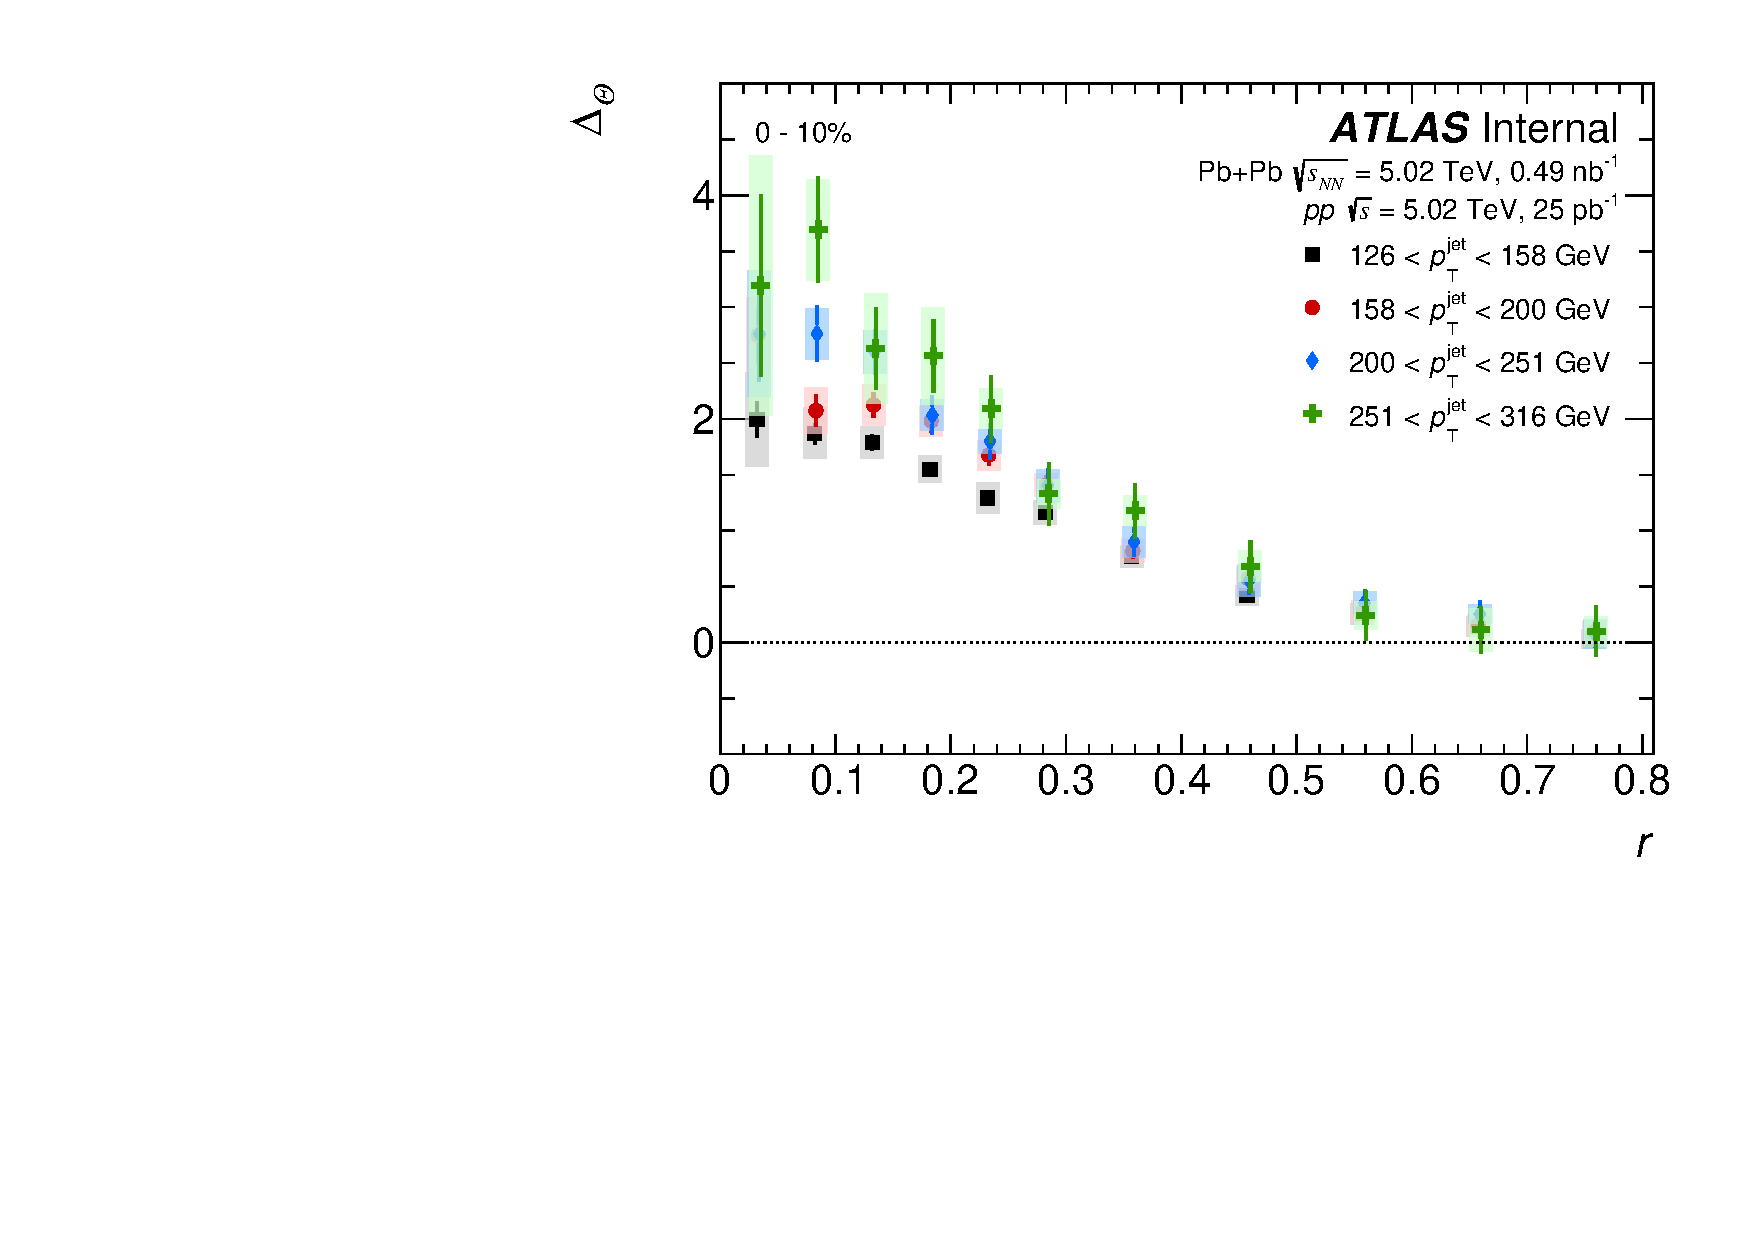
\includegraphics[width=0.36\textwidth]{results/DeltaDpT_lowpt_integ_cent0} &
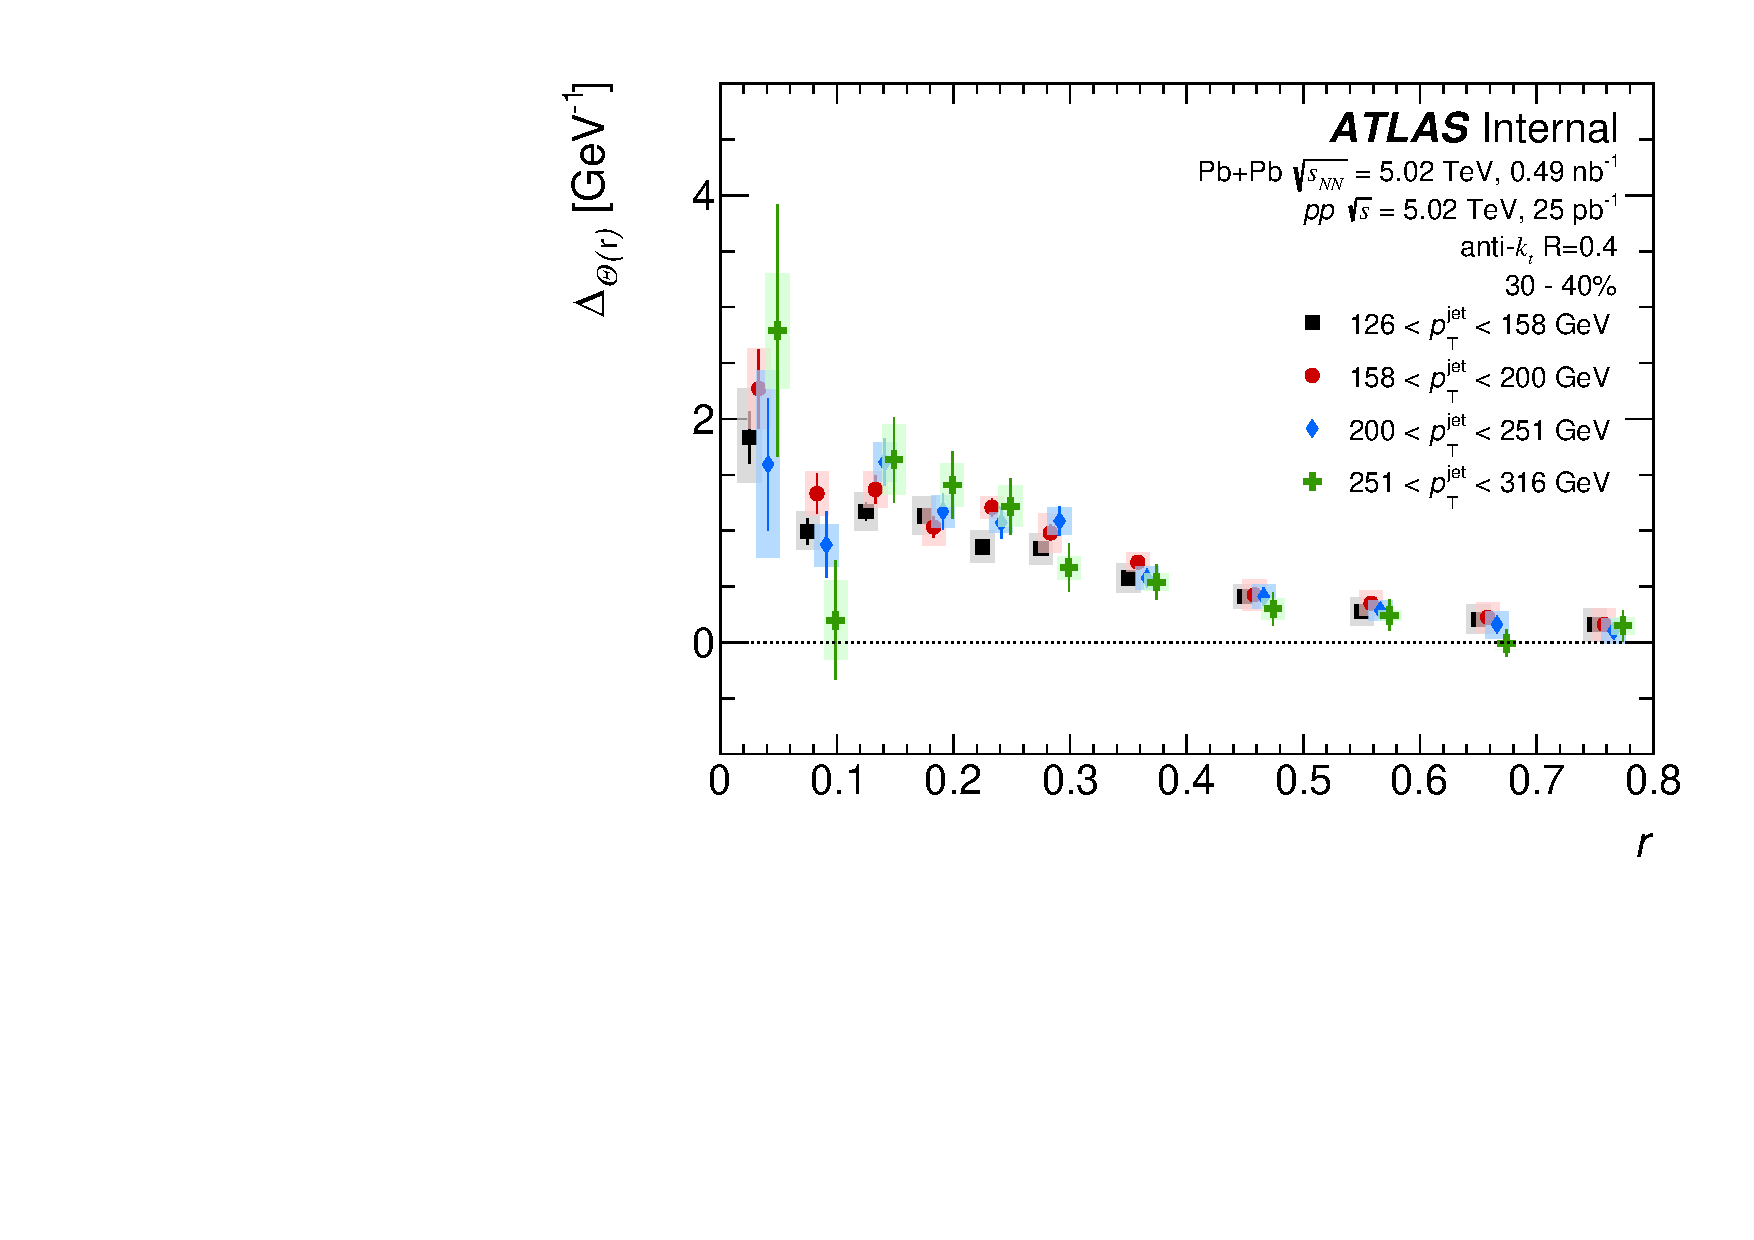
\includegraphics[width=0.36\textwidth]{results/DeltaDpT_lowpt_integ_cent3} &
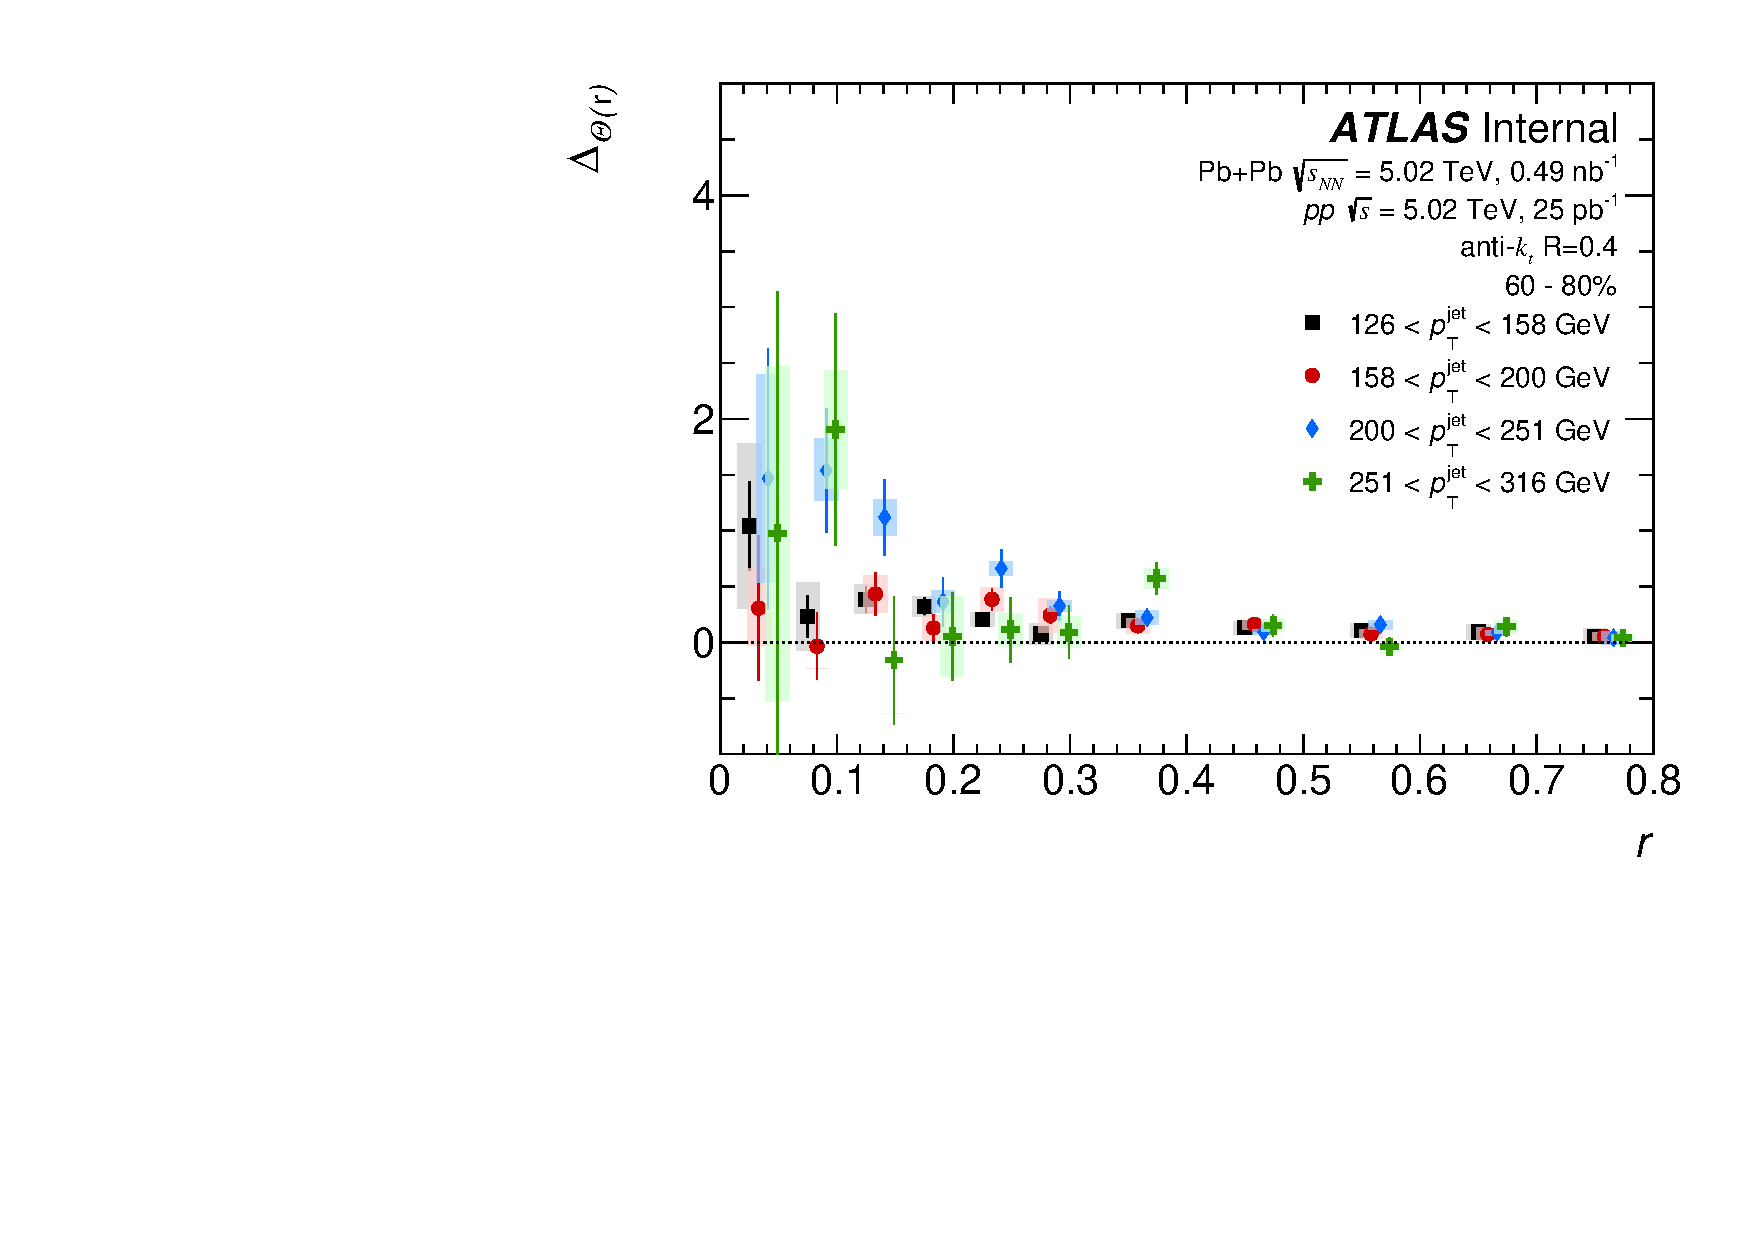
\includegraphics[width=0.36\textwidth]{results/DeltaDpT_lowpt_integ_cent5} \\
\end{tabular} }
\caption{\DeltaTheta\ as a function of \rvar\ for charged particles with \pt\ < 4 GeV  in four \ptjet\ selections: 126--158~\GeV, 158--200~\GeV, 200--251~\GeV, and 251--316~\GeV and three centrality selections: 0--10\% (left), 30--40\% (middle) and 60--80\% (right).
The vertical bars on the data points indicate statistical uncertainties while the shaded boxes indicate systematic uncertainties.
The widths of the boxes are not indicative of the bin size and the points are shifted horizontally for better visibility.}
\label{fig:deltaPdeltaT}
\end{figure}


\begin{figure}
\centerline{
\begin{tabular}{ccc}
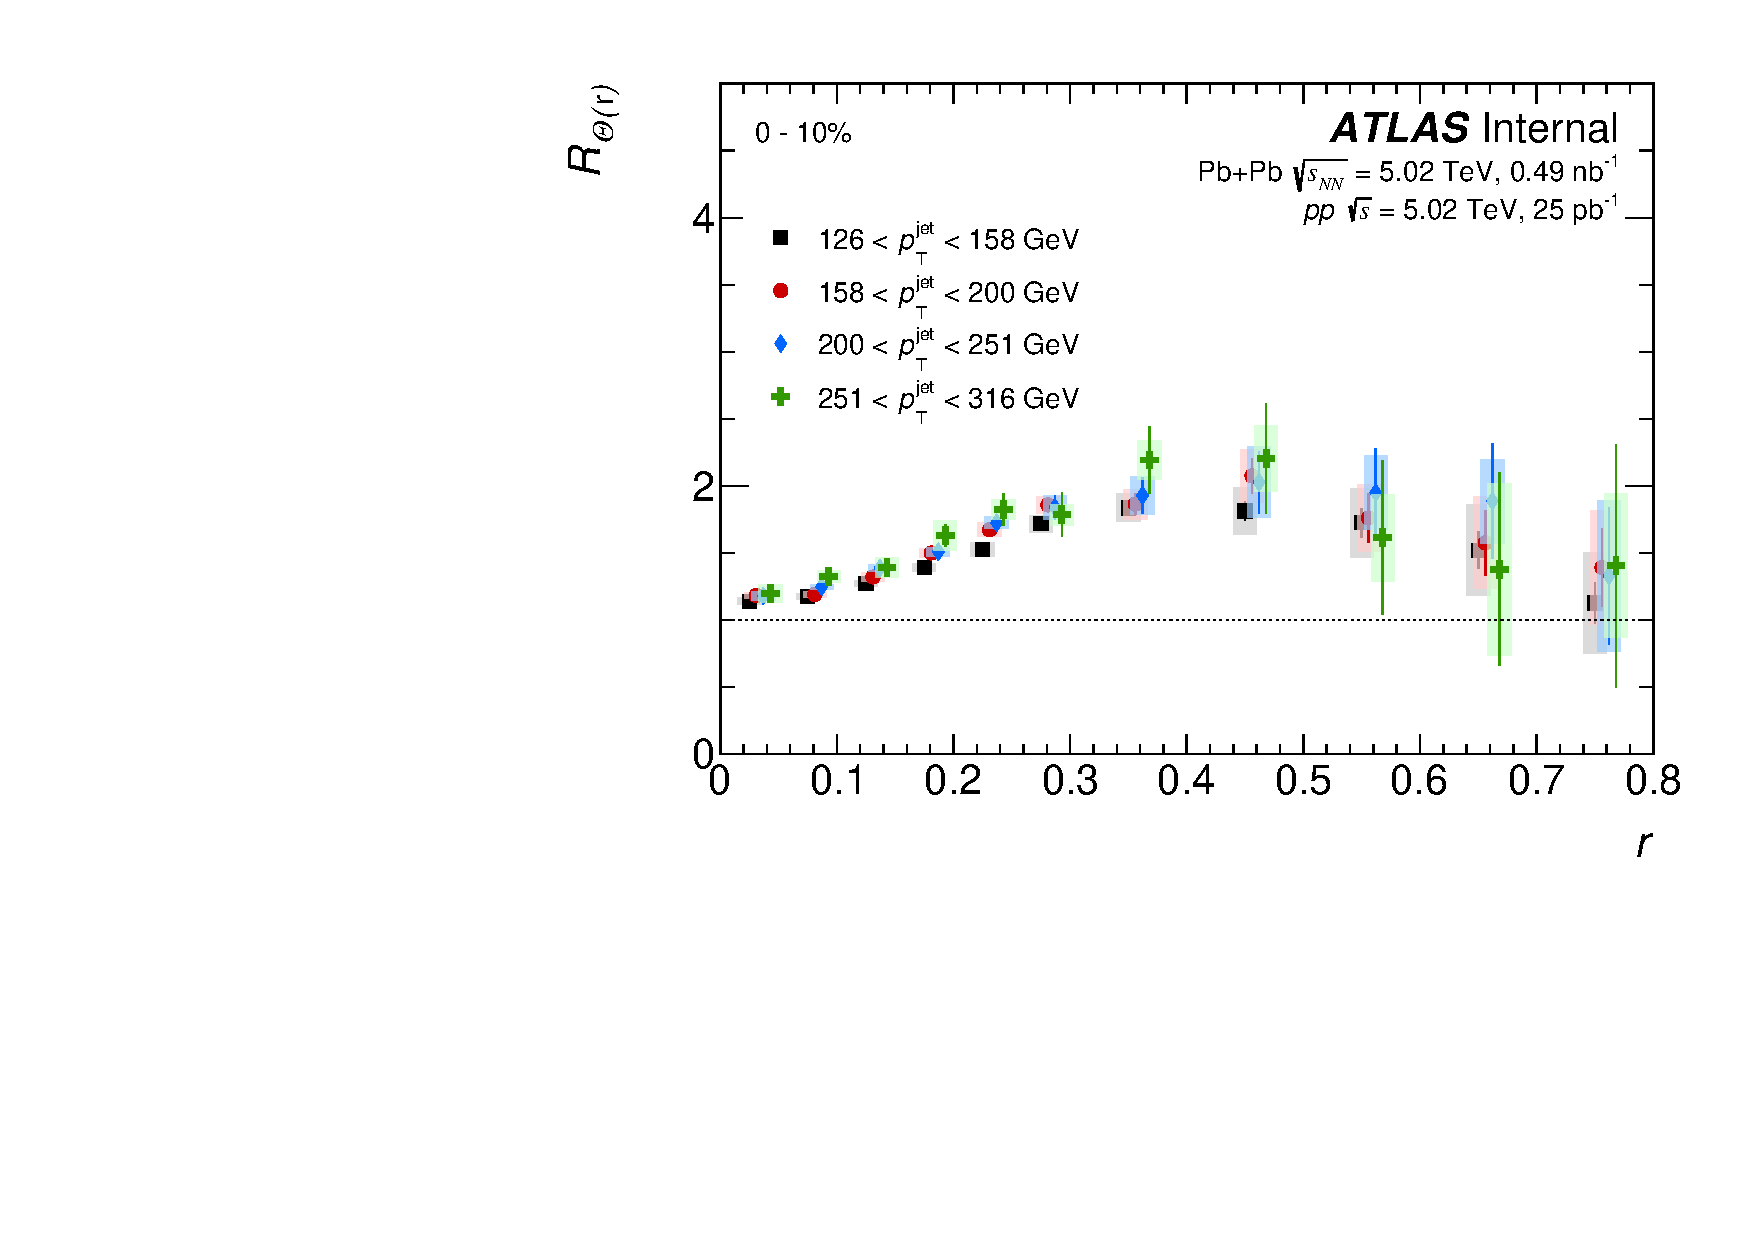
\includegraphics[width=0.36\textwidth]{results/RDpT_lowpt_integ_cent0} &
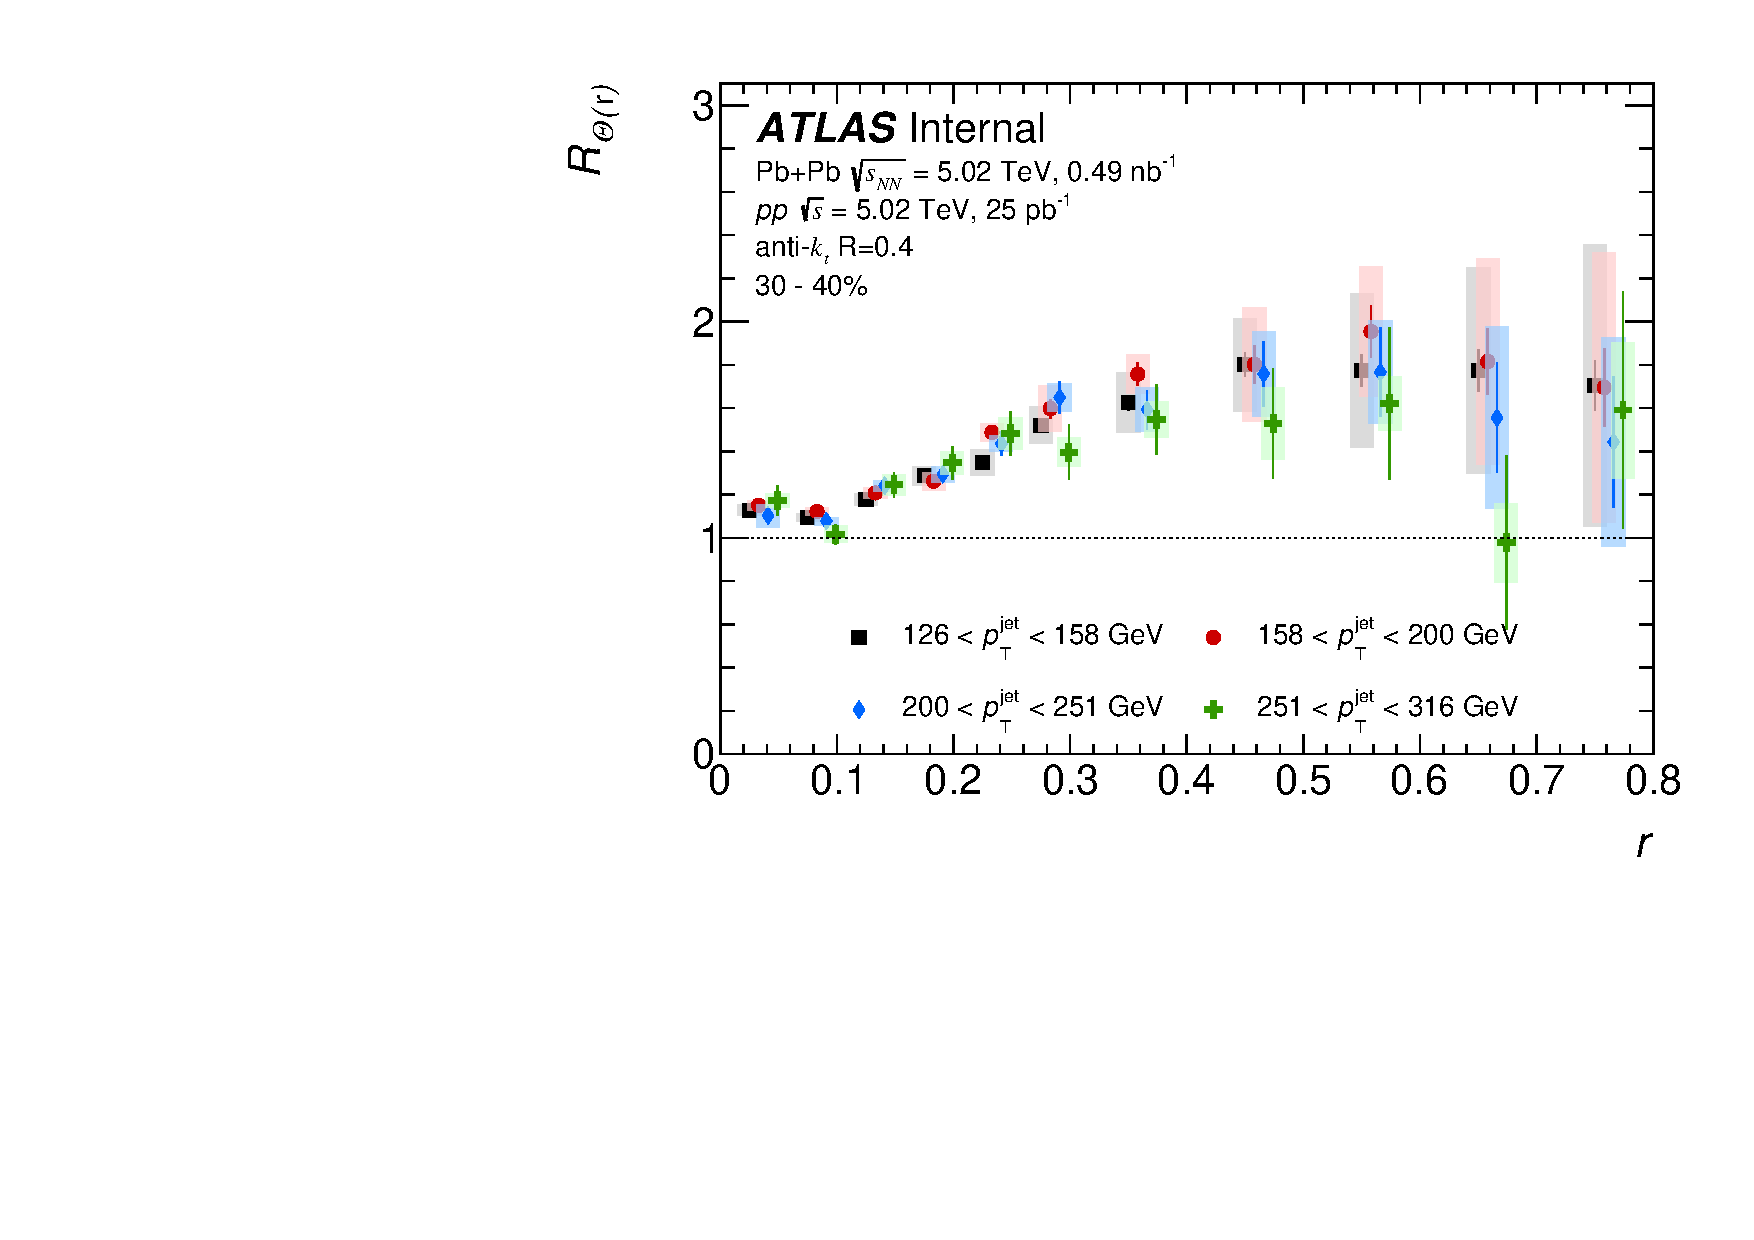
\includegraphics[width=0.36\textwidth]{results/RDpT_lowpt_integ_cent3} &
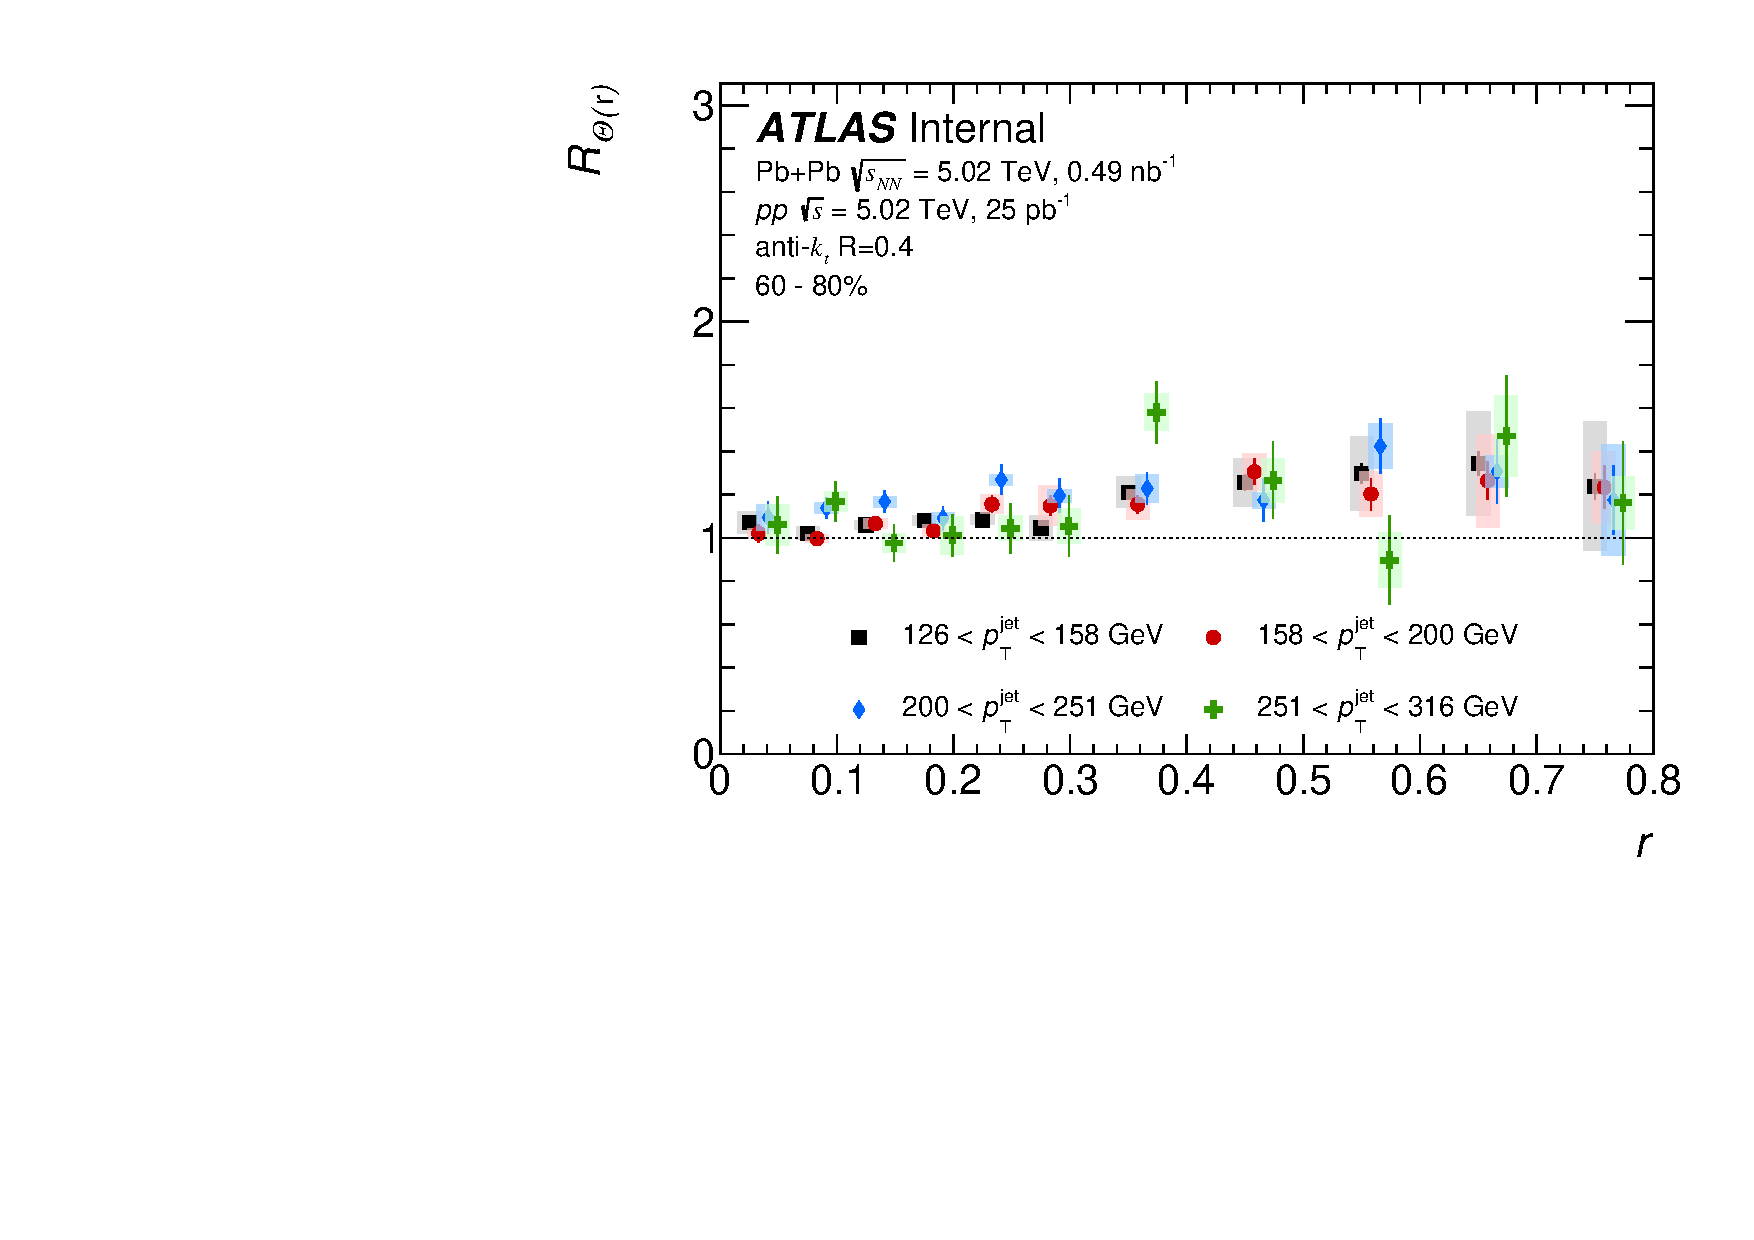
\includegraphics[width=0.36\textwidth]{results/RDpT_lowpt_integ_cent5} \\
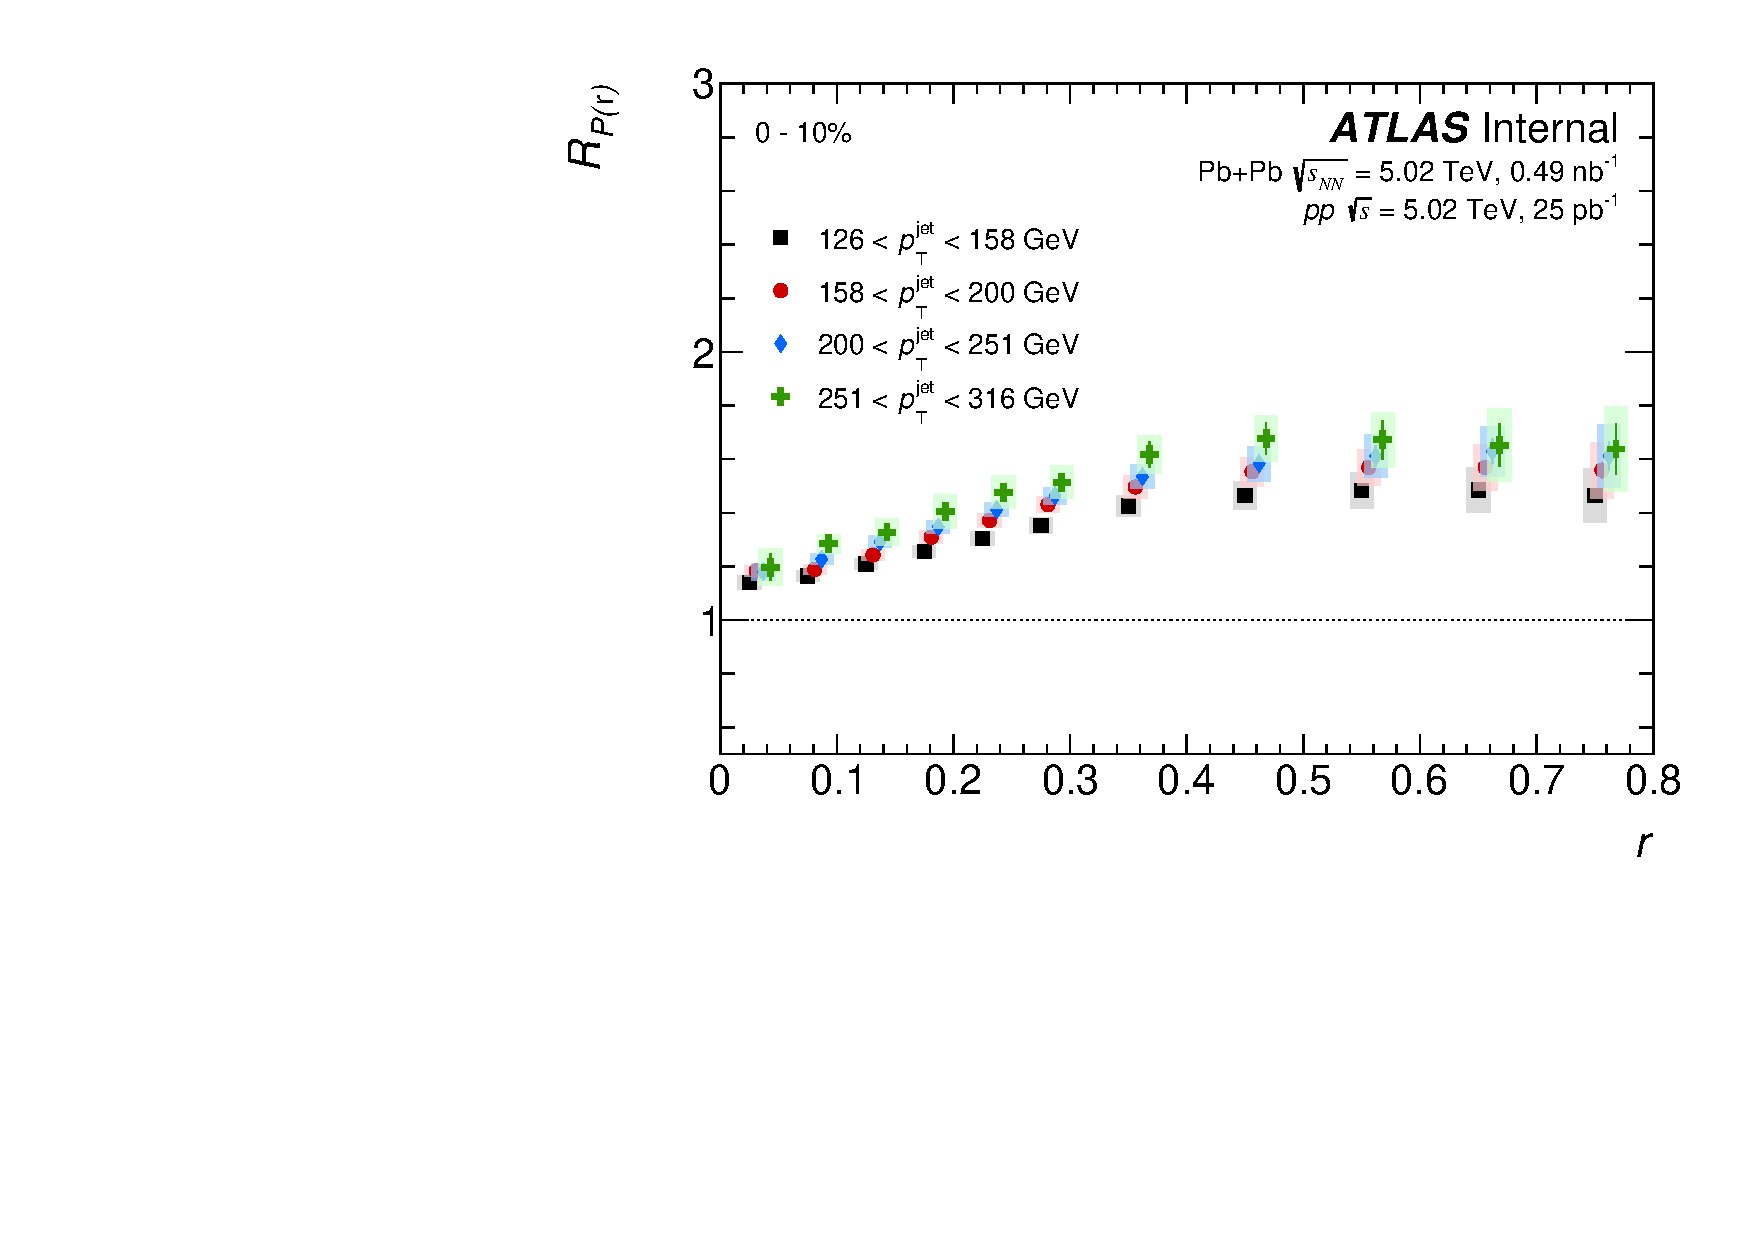
\includegraphics[width=0.36\textwidth]{results/RDpT_jetshape_cent0} &
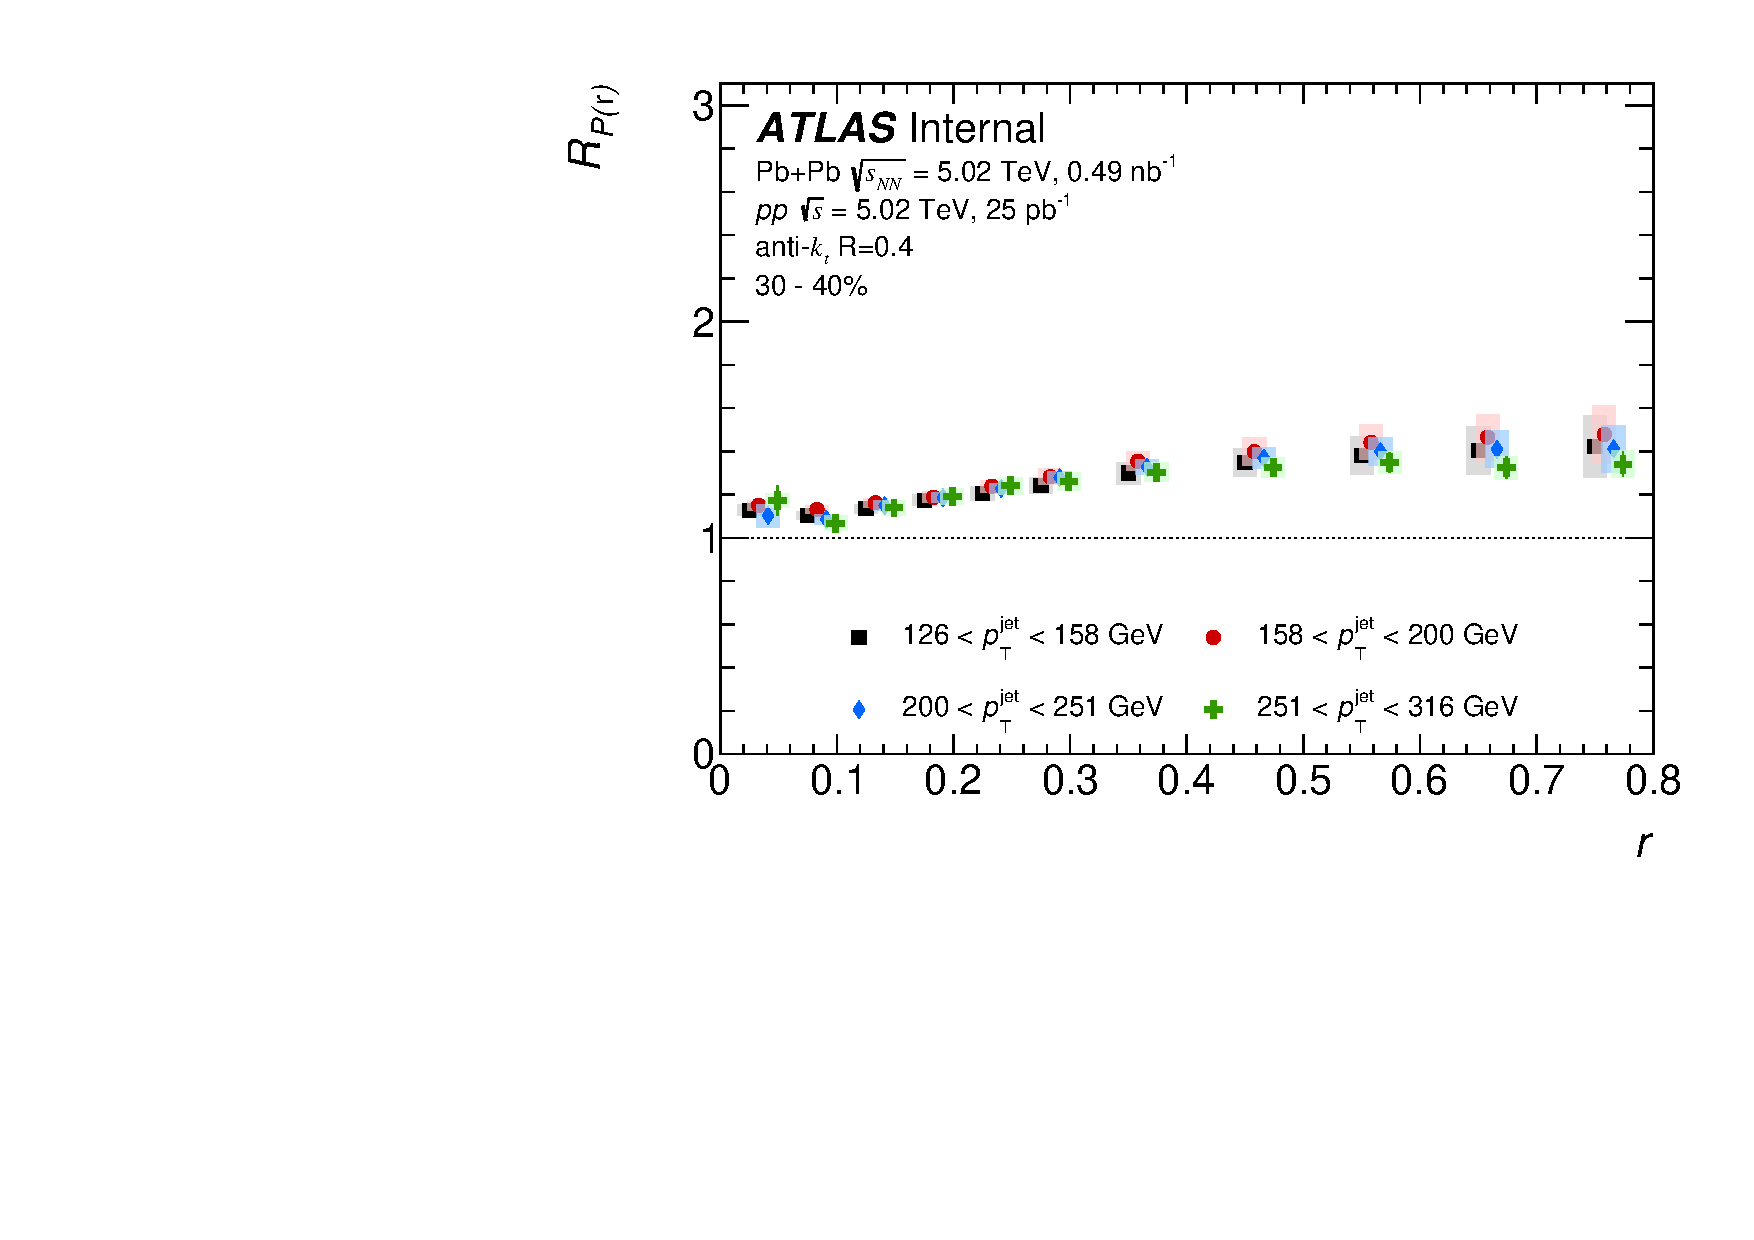
\includegraphics[width=0.36\textwidth]{results/RDpT_jetshape_cent3} &
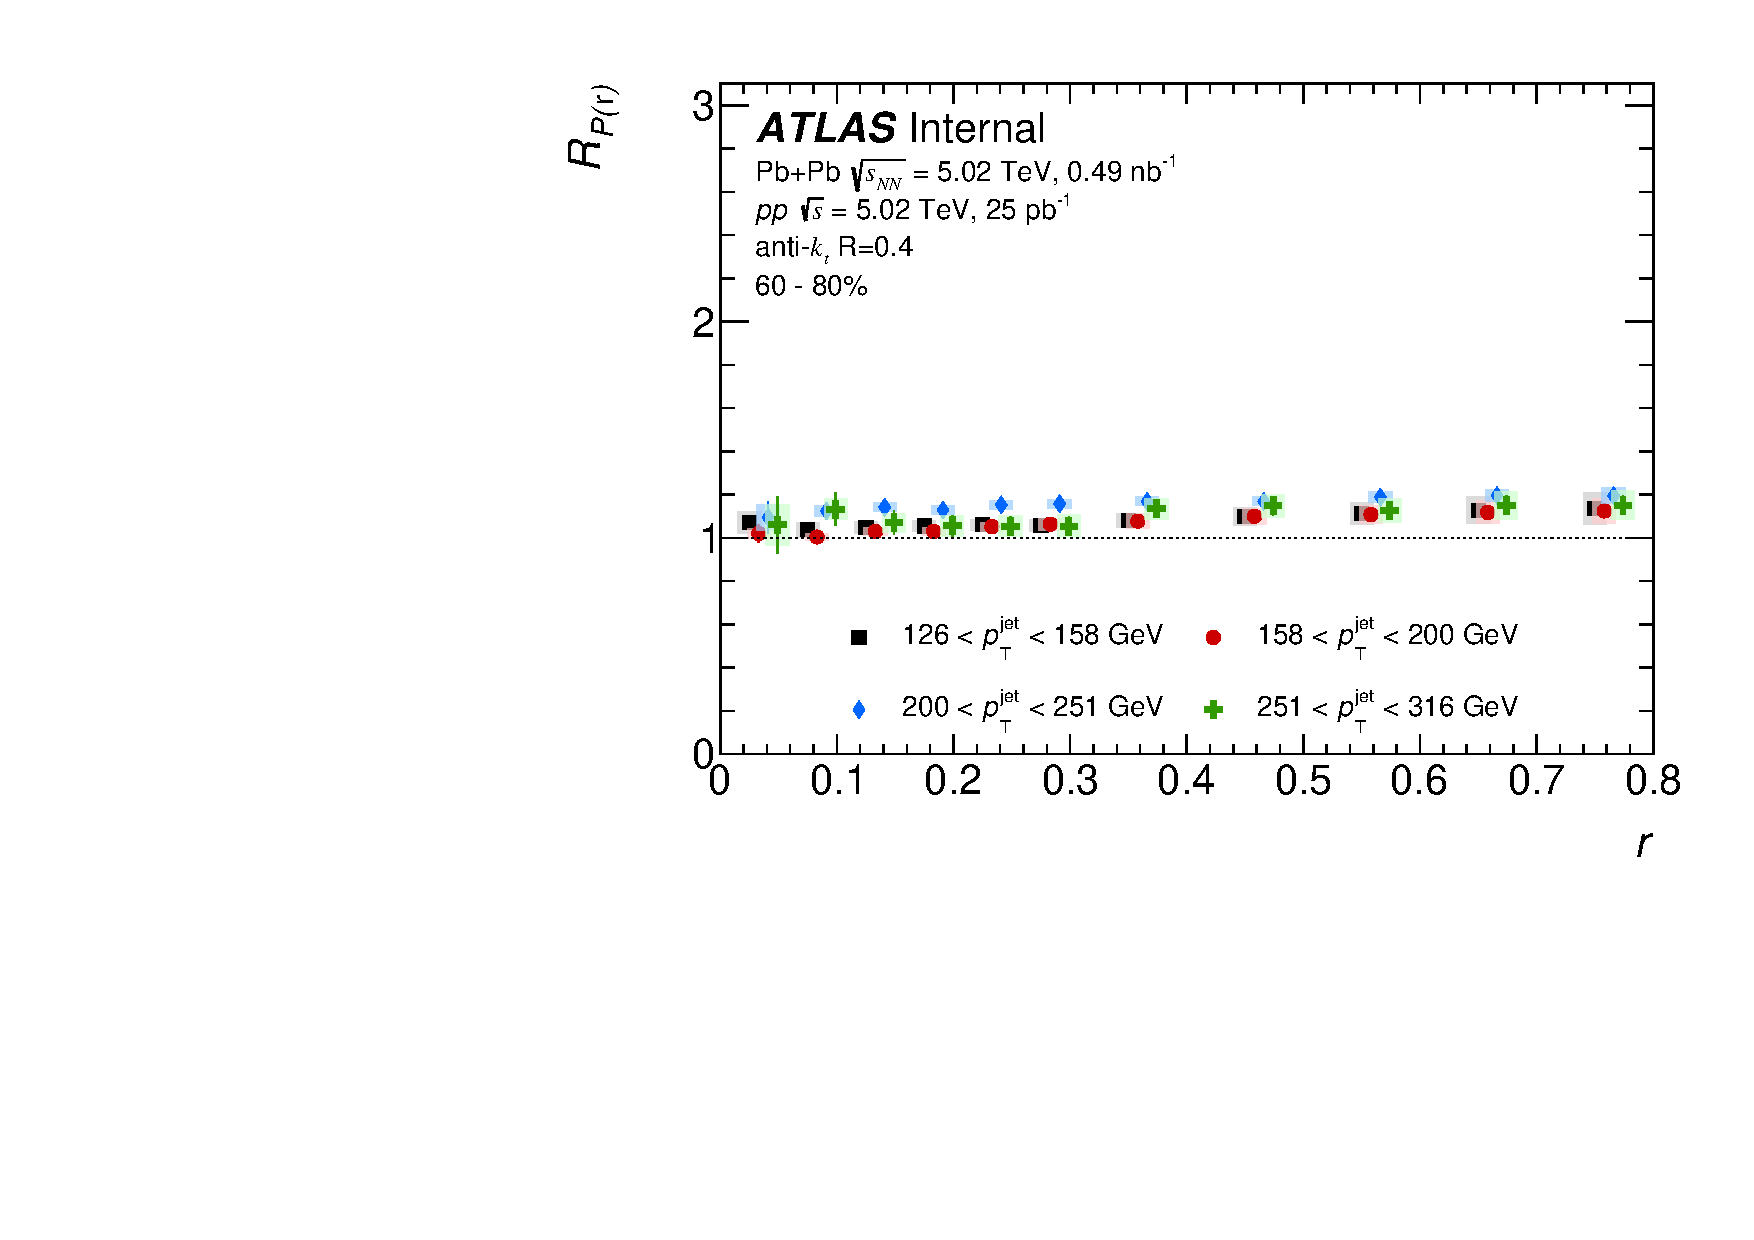
\includegraphics[width=0.36\textwidth]{results/RDpT_jetshape_cent5} \\
\end{tabular} }
\caption{\RTheta\ (top) and \RP\ (bottom) as a function of \rvar\ for charged particles with $\pt < 4$ GeV ranges in four \ptjet\ selections: 126--158~\GeV, 158--200~\GeV, 200--251~\GeV, and 251--316~\GeV\ and three centrality selections: 0--10\% (left), 30--40\% (middle) and 60--80\% (rights).
The vertical bars on the data points indicate statistical uncertainties while the shaded boxes indicate systematic uncertainties.
The widths of the boxes are not indicative of the bin size and the points are shifted horizontally for better visibility.}
\label{fig:RPRT}
\end{figure}


Figure~\ref{fig:RPRT} shows \RTheta\ and \RP\ for the following centrality intervals: 0--10\%, 30--40\% and 60--80\%.
The \RTheta\ distributions of the most central collisions show a maximum for $\rvar \sim 0.4$ and a flattening or a decrease for larger \rvar.
However, since \RTheta\ remains at or above unity for the full range of \rvar\ values presented, \RP\ shows no suppression with increasing \rvar\ over the entire measured range.
In more peripheral collisions the magnitude of the excess is reduced and the trends in \RTheta\ are less clear, however the slow increase of \RP\ is clearly seen for the 30--40\% central collisions.
The flattening of the \RP\ distributions at large distances demonstrates what while wider jets have a softer fragmentation and contain more particles with less \pt\ in \pbpb\ compared to \pp\ collisions \cite{Chesler2016, Hulcher:2017cpt}, this effect flattens out for jets with radius larger than 0.6.


%%%%
%These measurements show that the excess of particles with $\pt <$~4.0~\GeV\ observed in~\cite{Aaboud:2018hpb} extends
%outside the \RFour\ jet cone.
%The measured dependence of \RDptr\ suggests that the energy lost by jets through the jet quenching process is being transferred to particles with $\pt <$~4.0~\GeV\ at larger radial distances from the jet axis.
%This is qualitatively consistent with theoretical calculations \mbox{\cite{Blaizot:2014ula}}.
%Additionally, these observations are in agreement with the previous measurement of jet fragmentation functions \cite{Chatrchyan:2014ava, Sirunyan:2018jqr, Aaboud:2017bzv, Aaboud:2018hpb} and may indicate the dependence of the response of the hot dense matter to the momentum of a jet passing through it.
%%%%%

\FloatBarrier
